\documentclass[10pt,twoside,openright,titlepage]{ce}

% =Imports===============================================================================
\usepackage[]{tcolorbox}
\usepackage[]{amsmath,amssymb,amsthm}
\usepackage[]{graphicx}
\usepackage[]{color}
\usepackage[]{listings}
\usepackage[]{hyperref}
\usepackage[]{nielsformat}
\usepackage[]{subcaption}
\usepackage[]{tikz}
\usepackage[]{tikz-3dplot}
\usepackage[]{pgfplots}
\usepackage[]{pgfplotstable}
\usepackage[]{multirow}

\pgfplotsset{compat=1.16}
\usetikzlibrary{pgfplots.groupplots}

% =Definitions===========================================================================
\usepackage[]{nielstex}
\usepackage[]{nielstikz}

% Define plot command
\begin{tikzpicture}
    \begin{axis}[xlabel=$Q$, ylabel=PESQ]
        \addplot [color=blue, mark=*, error bars/.cd, y dir=both, y explicit]
        table [x expr=\thisrow{Q}, y expr=\thisrow{A__0.wav__target_reconstruction_pesq_mean}, 
            y error expr=\thisrow{A__0.wav__target_reconstruction_pesq_std}, col sep=comma] 
            {data/constraining.csv};
        \addplot [color=red, mark=*, error bars/.cd, y dir=both, y explicit]
        table [x expr=\thisrow{Q}, y expr=\thisrow{A__0.wav__target_result_pesq_mean}, 
            y error expr=\thisrow{A__0.wav__target_result_pesq_std}, col sep=comma] 
            {data/constraining.csv};
    \end{axis}
\end{tikzpicture}


% Thesis specific definitions
\newcommand{\za}{\mathcal{A}}
\newcommand{\zb}{\mathcal{B}}
\newcommand{\zz}{\mathcal{Z}}

% For presenting the research questions, some stuff I stole of SO
% NOTE: not used as of now
\usepackage{enumitem}
\newlist{questions}{enumerate}{2}
\setlist[questions,1]{label=RQ\arabic*.,ref=RQ\arabic*}
\setlist[questions,2]{label=\thequestionsi.\arabic*,ref=\thequestionsi(\alph*)}

% =Document Attributes===================================================================
\msctitle{Sound Zones with a Cost Function based on Human Hearing}
\mscsubtitle{}
\msckeywords{perceptual sound zones, sound field control, perceptual models, pressure matching}
\mscauthor{Niels Evert Marinus de Koeijer B.Sc.}
\msccity{Delft}
\msccountry{The Netherlands}
\mscnumber{??}
\mscdate{September 15, 2021}
\major{Electrical Engineering}
\mscinstitute{Delft University of Technology}
\mscfaculty{Electrical Engineering, Mathematics and Computer Science}
\mscdepartment{Microelectronics \& Computer Engineering}
\mscgroup{Circuits and Systems}
\chairperson{dr.ir. R.C. Hendriks}
\memberone{dr. M. Mastrangeli}
\membertwo{dr. M. Bo M\o ller}
\memberthree{dr. P. Mart\'{\i}nez-Nuevo}
\advisorone{dr. J. Mart\'{\i}nez-Casta{\~n}eda }

% =Abstract==============================================================================
\def\ABSTRACT{}

% =Document==============================================================================
\begin{document}

% =Front Pages===========================================================================
\frontmatter
\makecover
\maketitle
\makesignature
% Thesis Abstract ----------------------------------------------
%
\nonumchapter{Abstract}%
%
%
% The abstract you put in the preamble will appear here:
%
\ABSTRACT%
%
\cleardoublepage%

\nonumchapter{Acknowledgments}
\vskip 1cm
I would like to thank \FIRSTADVISOR, \SECONDMEMBER, \CHAIRPERSON, and \THIRDMEMBER\ for all their help and support during the project.
A special thanks to \SECONDMEMBER\ for often pushing me in the right direction through our numerous white board sessions.
Secondly, I would also like to especially thank \FIRSTADVISOR for being a major help during, and outside of the project.

In addition to this, I would like to thank Cassandra Gr\"utzner and especially 
Dorottya Hauk for their help proof reading the thesis 
and for many good times during the project.

\vskip 2cm
\noindent \AUTHOR \\
\PLACE \\
\DATE

\tableofcontents
% \listoffigures
% \listoftables
\mainmatter

% =Content===============================================================================
\chapter{Introduction}
\label{ch:introduction}
\begin{tikzpicture}
    \begin{groupplot}[group style={group size=1 by 3, vertical sep=2cm}]
        \nextgroupplot[xlabel={Time [samples]}, ylabel={$t^{(m)}[n]$ [SPL]}, ylabel near ticks, 
        title={Target Sound Pressure for Control Point $m\in A$}, scale only axis, 
        height=3cm, width=9cm, xmin=5000, xmax=6400, xtick={5000, 5200, 5400, 5600, 5800, 6000, 6200, 6400},
        ymin=-0.5, ymax=0.5]
        \addplot [color=red, error bars/.cd, y dir=both, y explicit]
        table [x expr=\thisrow{samples}, y expr=(\thisrow{audio} / 32787), col sep=comma] 
            {data/target.csv};
       \addplot [samples=50, smooth, name path=H11] coordinates {(5500,-0.5) (5500,0.5)};
       \addplot [samples=50, smooth, name path=H12] coordinates {(6200,-0.5) (6200,0.5)};
       \addplot [fill opacity=0.05] fill between [of=H11 and H12];

        \nextgroupplot[xlabel={time [samples]}, ylabel={$p_\zb^{(m)}[n]$}, ylabel near ticks, 
        title={Perceptual Achieved Dark Zone Sound Pressure for Control Point $m\in A$}, scale only axis, 
        height=3cm, width=9cm, xmin=5000, xmax=6400, xtick={5000, 5200, 5400, 5600, 5800, 6000, 6200, 6400},
        ymin=-0.5, ymax=0.5]
        \addplot [color=red, error bars/.cd, y dir=both, y explicit]
        table [x expr=\thisrow{samples}, y expr=(\thisrow{audio} / 32787), col sep=comma] 
            {data/per_leakage.csv};
       \addplot [samples=50, smooth, name path=H11] coordinates {(5500,-0.5) (5500,0.5)};
       \addplot [samples=50, smooth, name path=H12] coordinates {(6200,-0.5) (6200,0.5)};
       \addplot [fill opacity=0.05] fill between [of=H11 and H12];

        \nextgroupplot[xlabel={time [samples]}, ylabel={$p_\zb^{(m)}[n]$}, ylabel near ticks, 
        title={Reference Achieved Bright Zone Sound Pressure in Control Point $m\in A$}, scale only axis, 
        height=3cm, width=9cm, xmin=5000, xmax=6400, xtick={5000, 5200, 5400, 5600, 5800, 6000, 6200, 6400},
        ymin=-0.5, ymax=0.5]
        \addplot [color=red, error bars/.cd, y dir=both, y explicit]
        table [x expr=\thisrow{samples}, y expr=(\thisrow{audio} / 32787), col sep=comma] 
            {data/ref_leakage.csv};
       \addplot [samples=50, smooth, name path=H11] coordinates {(5500,-0.5) (5500,0.5)};
       \addplot [samples=50, smooth, name path=H12] coordinates {(6200,-0.5) (6200,0.5)};
       \addplot [fill opacity=0.05] fill between [of=H11 and H12];
    \end{groupplot}
\end{tikzpicture}

\section{Preface}
\label{ch:introduction:preface}
Sound systems are used world wide to fill rooms with enjoyable audio content. 
Problems arise however when multiple people in the same room want to enjoy different audio content at the same time.

For example, one person may want to enjoy a movie on television, while another may want to listen to their music.
If they are in the same room, their desires clash: neither person can fully enjoy their chosen activity without disturbing
the other.
In short, the interference of multiple source of audio leads to a situation where both individual experiences are diminished.

In recent years, attempts have been made to solve this problem by controlling the spatial reproduction of sound in such
a way that different areas in a room have distinct content.

One class of algorithms that attempt to do so are sound zone algorithms~\cite{betlehem2015personal}.
Sound zone algorithms partition the space of the room into multiple so-called sound zones.
Each sound zone is assigned different audio content.
The sound zone algorithms decides how to use the loudspeakers of the sound system to reproduce said audio content in every zone.
Using the principals of constructive and destructive interference, this is done in such that there is minimal interference between zones.
That is to say: the audio content of each zone is not audible in the others.

In the previously listed example, one zone would contain the audio of a movie and another zone would contain music.
An image depicting the situation is given in \autoref{fig:introduction:motivation:concept}.
The sound zone algorithm determines how to best use the sound system to reproduce these two zones.
In the ideal case, both people can now enjoy the full potential of their audio content, without bothering one another.

\begin{figure}[]
    \centering
    \scalebox{1.0}{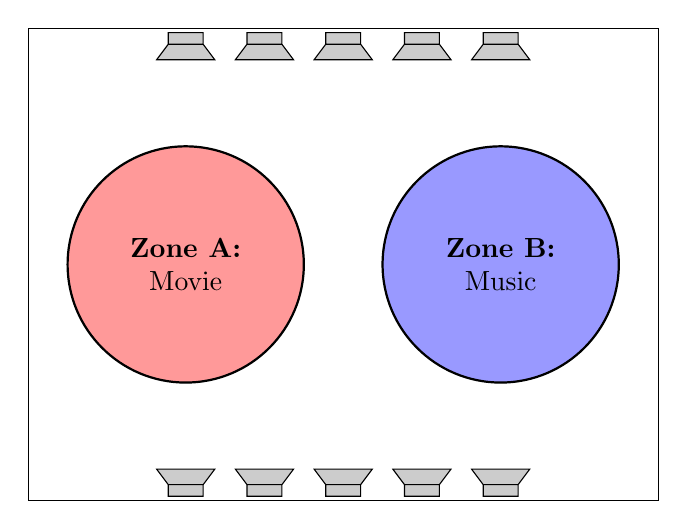
\begin{tikzpicture}
    \tikzset{
      Speaker/.pic={
        \filldraw[fill=gray!40,pic actions] 
        (-15pt,0) -- 
          coordinate[midway] (-front) 
        (15pt,0) -- 
        ++([shift={(-6pt,8pt)}]0pt,0pt) coordinate (aux1) -- 
        ++(-18pt,0) coordinate (aux2) 
        -- cycle 
        (aux1) -- ++(0,6pt) -- coordinate[midway] (-back) ++(-18pt,0) -- (aux2);
      }
    }

    \draw [draw=black] (0,0) rectangle (8,6);

    % Speakers on the top wall
    \pic[scale=0.7] at (2, 5.6) {Speaker};
    \pic[scale=0.7] at (3, 5.6) {Speaker};
    \pic[scale=0.7] at (4, 5.6) {Speaker};
    \pic[scale=0.7] at (5, 5.6) {Speaker};
    \pic[scale=0.7] at (6, 5.6) {Speaker};

    % Speakers on the bottom wall
    \pic[rotate=180, scale=0.7] at (2, 0.4) {Speaker};
    \pic[rotate=180, scale=0.7] at (3, 0.4) {Speaker};
    \pic[rotate=180, scale=0.7] at (4, 0.4) {Speaker};
    \pic[rotate=180, scale=0.7] at (5, 0.4) {Speaker};
    \pic[rotate=180, scale=0.7] at (6, 0.4) {Speaker};

    \draw[opacity=0.4, fill=blue] (6,3) circle[radius=1.5];
    \draw[thick] (6,3) circle (1.5) node[align=center] {\textbf{Zone B:}\\Music};
    \draw[opacity=0.4, fill=red]  (2,3) circle[radius=1.5];
    \draw[thick] (2,3) circle (1.5) node[align=center] {\textbf{Zone A:}\\Movie};
\end{tikzpicture}
}
    \caption{A room containing a sound system consisting of an array of loudspeakers and two zones.
                The goal of the sound zone algorithm is to control the sound system in such a way that the red zone
                contains the audio of a movie, and the blue zone contains the music.}
    \label{fig:introduction:motivation:concept}
\end{figure}

In practice however, the sound zone algorithm will not always do a perfect job.
The performance of algorithms depends on the environment and the available sound system.
Depending on the situation, the interference between zones can typically only be reduced by so much.
As such, audio content of one zone is often still audible in other zones.

Improving sound zone algorithms is thus still an active topic of research.
One recent approach is to include a model of the human auditory system, which models how sound is perceived by humans.
Typically, sound zone algorithms use sound pressure, which is the physical phenomenon of sound.
Sound pressure doesn't always capture what is important for the perception of sound.
As such, including a perceptual model may allow the algorithm to focus on the parts of the audio content
that matter perceptually.

Early results show that the perceptual sound zone approach is promising.
Recent work by Donley et al. explored including the absolute threshold of hearing, which models the lowest sound pressure
humans can hear, into sound zone algorithms.
This pursuit found an increased quality of the reproduced audio in the zones~\cite{donley2015multizone}.
Other work by Lee et al. showed that including a perceptually-motivated weighting in the sound zone algorithm outperforms 
traditional algorithms~\cite{lee2019towards,lee2020signal}.

This work will seek to further explore this perceptual approach by proposing a novel perceptual sound zone algorithm and exploring
the possible benefits.

\newpage
\section{Objectives and Organization}
\label{ch:introduction:objectives}
This section will state the goals of the thesis and organization of the rest of this document.
Als stated in the motivation, the goal of the thesis is to construct a perceptual sound zone algorithm.
The central question in this thesis is: 

{\centering\textit{``How can perceptual models of the human auditory system be used to improve sound zone algorithms?''}}

This question is answered in three steps. 
First, a perceptual model is selected in \autoref{ch:perceptual}.
Next, a sound zone algorithm is selected in \autoref{ch:sound_zone}.
Finally, the two are combined and the resulting algorithm is evaluated in \autoref{ch:perceptual_sound_zone}.
The organization of the three chapters is given below.

\subsection{Search and Implementation of a Perceptual Model}
\label{ch:introduction:objectives:perceptual}
In order to construct a perceptual sound zone algorithm, a perceptual model is required.
This begs the question: ``What perceptual models exist?''.
To answer this question, this chapter starts with a summary of necessary psycho-acoustics background in 
\autoref{ch:perceptual:background} followed by a literature review into state of the art perceptual models
in \autoref{ch:perceptual:review}.

To select a perceptual model suitable for combination with a sound zone algorithm, one must consider what 
desired properties of such a model.
These criteria and the resulting selection of one of the perceptual models from the 
literature review is given in \autoref{ch:perceptual:selection}.

The selected perceptual model is then discussed in greater detail in \autoref{ch:perceptual:implementation}. 
Here, implementation details are given and analysis are performed to give the reader an intuition into the model.

\subsection{Search and Implementation of a Sound Zone Approach}
\label{ch:introduction:objectives:sound_zone}
After selecting a perceptual model, a suitable sound zone approach must be selected.
Before determining which sound zone approaches are suitable, a literature review is performed in
\autoref{ch:sound_zone:approach_review} to document what sound zone approaches exist.

The perceptual model will impose certain constraints on which sound zone algorithm is best suited for integration.
As such, \autoref{ch:sound_zone:approach_selection} will reflect on these constraints to select one of the documented
sound zone approaches as the most promising for integration.

The sections that follow will discuss implementation details of the selected sound zone approach.
In \autoref{ch:sound_zone:data_model} a general sound zone data model will be given, formalizing the sound zone problem
and laying the mathematical foundation.
This mathematical foundation is then used in \autoref{ch:sound_zone:approach_implementation} and 
\autoref{ch:sound_zone:block_based} to derive a sound zone algorithm based on the selected sound zone approach.

The derived sound zone algorithm will form the foundation on which the perceptual sound zone algorithm will be built.
In addition to this, it will serve as a reference implementation with which the perceptual sound zone algorithm
can be compared.

\subsection{Implementation of a Perceptual Sound Zone Algorithm}
\label{ch:introduction:objectives:perceptual_sound_zone}


\chapter{Perceptual Model Review and Implementation}
\label{ch:perceptual}
% \section{Introduction}
% \label{ch:perceptual:introduction}
% The goal of this chapter is to find a suitable perceptual algorithm for the creation of a perceptual sound zone algorithm.
This chapter is structured as follows.

The chapter will begin in \autoref{ch:perceptual:background} with some background information on the human auditory system.
This is done to ensure that the reader has the knowledge to understand the perceptual aspects of the thesis.

Next, with the necessary psycho-acoustical background in place, a literature review into perceptual models is given in \autoref{ch:perceptual:review}.
The purpose of this review is to document candidates for the perceptual model that will be used in the perceptual sound zone algorithm.
In addition to this, the reviewed models could also serve as potential candidates for use in the evaluation 
of the perceptual sound zone algorithm that will be proposed in \autoref{ch:perceptual_sound_zone}.

To perform the selection of a perceptual model from the candidates discussed in the literature review, 
criteria reflecting desirable properties for the model for use in sound zones are be defined in \autoref{ch:perceptual:selection}. 
The criteria are then used to select a perceptual model.

Afterwards, the selected perceptual model is discussed in more detail in \autoref{ch:perceptual:implementation} by stating implementation 
details and describing its behavior.
The chapter will then wrap up with its conclusions in \autoref{ch:perceptual:conclusion}.

% \newpage
\section{Perceptual Background}
\label{ch:perceptual:background}
In the field of psycho-acoustics significant research has been done in characterizing the auditory 
perception and time-frequency
analysis capabilities of the human ear~\cite{painter2000perceptual}.
From this understanding, several perceptual models have been proposed which aim to model the 
perception of auditory stimuli by humans~\cite{van2005perceptual}.

Perceptual models are employed for various purposes.
Objective audio quality measures, for example, are perceptual models which aim to predict the perceived quality of audio~\cite{torcoli2021objective}.
In another example, perceptual audio coding uses models of auditory perception to minimize the perceived artifacts introduced when
performing the compression of audio~\cite{herre2019psychoacoustic}.

In general, many perceptual models operate on a time-frequency internal-ear representation of the input stimuli, obtained by applying an analysis filter bank. 
Among other effects, the filtering performed by the human ear is often taken 
into account at this stage~\cite{van2005perceptual, taal2012low}.
This representation is then used to determine its perceptually relevant aspects 
of the input stimuli~\cite{herre2019psychoacoustic}.

One aspect often used in perceptual models are the various auditory masking properties of the 
input stimuli~\cite{herre2019psychoacoustic}.
In general, auditory masking refers to the effects one sound has on the perception of other sounds~\cite{painter2000perceptual}.
In simultaneous masking, for example, one loud tone may overpower a tone of a similar frequency, rendering the 
latter tone inaudible~\cite{painter2000perceptual}.

Another aspect that is often used is the ``threshold of hearing'', which determines the minimum sound pressure level that can be perceived by a human~\cite{herre2019psychoacoustic}.
Combining this principle with the masking properties, one can define the ``masking threshold'' of input stimuli.
This threshold determines the sound pressure level required for other stimuli to be audible to a human observer in the presence of the input stimuli~\cite{painter2000perceptual} and is often used in perceptual 
models~\cite{van2005perceptual, taal2012low}. 
For example, the threshold of hearing is used in perceptual audio coding to 
make the coding artifacts inaudible~\cite{herre2019psychoacoustic}.

This chapter will motivate the use of the ``Par distortion detectability'' as the perceptual model used in perceptual sound zone algorithm framework proposed in \autoref{ch:sound_zone}, which is subsequently used in \autoref{ch:perceptual_sound_zone} to propose two perceptual sound zone algorithms.
In doing so, several other perceptual measures are discussed in detail, some of which are used in \autoref{ch:results} to evaluate the performance of the proposed algorithms.

The structure of this chapter is given as follows.
\begin{itemize}
    \item This chapter begins with \autoref{ch:perceptual:review} which documents a review of 
        possible candidate perceptual models from literature for use in the perceptual sound zone framework. 
    \item Next, \autoref{ch:perceptual:selection} motivates the selection of one of the reviewed candidates, 
        namely the ``Par distortion detectability'', as the perceptual model for use in the 
        proposed perceptual sound zone framework.
    \item Finally, the implementation and behavior of the ``Par distortion detectability'' is discussed in more detail in 
        \autoref{ch:perceptual:implementation}.
\end{itemize}

\newpage
\section{Review of Perceptual Models from Literature}
\label{ch:perceptual:review}
This section will document a literature review into perceptual models of the human auditory system.
As stated in the introduction, this literature review is performed to determine which perceptual models are currently 
available in the state of the art.
This review will then be later used in \autoref{ch:perceptual:selection} to select a perceptual model most 
suitable for integration into a sound zone algorithm.

For this literature review, the goal was to document the perceptual models that were either promising for 
the integration into algorithms or for evaluating the quality of the output of algorithms.
These are models that attach some ``score'' or ``rating'' to the perceptual quality of input signals.
These ratings can then be used in algorithms to obtain an optimal rating through optimization, or to determine
the quality of results from later algorithms.

As such, the focus of the literature review is not on the latest findings in psycho-acoustics, or models 
that accurately emulate the behavior of the human ear, such as the Dau model.
Instead, two categories of perceptual models are considered.

First, ``Objective Measures'', which are discussed in \autoref{ch:perceptual:review:objective}, which attempt to predict
the perceptual quality ratings found in listening tests. 
And ``Audio Coding'' models, discussed in \autoref{ch:perceptual:review:audio_coding}, which are used to quantify how
perceptually audible the artifacts of compression in audio are.

\subsection{Objective Measures}
\label{ch:perceptual:review:objective}
In order to determine the perceived quality of audio one approach is to use listening tests.
These are tests in which subjects are asked to rate a property (or properties) of a set of audio stimuli.
One example where these tests are performed is for the evaluation of listening aids, where they are used determine 
the speech intelligibility~\cite{taal2011algorithm}.
Other examples include determining which loudspeaker has the best perceived sound quality.

Performing listening tests is however often cumbersome due to the large amount of human labour involved.
This motivates the use of objective quality measures, which attempt to predict the outcomes of these listening tests.
This is very useful for algorithm developers for example, as they can get an indication of how well they are doing
without having to perform a cumbersome test.
Note however that a objective quality measure does not replace a listening test: it can only be used to give an 
indication.

The objective measure that will be considered take a reference and degraded audio stimuli as inputs.
The quality of the degraded audio stimuli is then determined by the measure.
For example, a speech intelligibility measure will determine the intelligibility of a degraded audio file.

These objective quality measures are promising for integration into sound zone algorithms as they summarize the 
quality of a signal into a single value, which can be potentially optimized for. 
It stands to reason that if an objective quality measure correlates with audio quality, optimizing over such a measure
could improve sound zone algorithms.

As such, this section will explore various objective measures.
This will be done by considering various different objective measure classes. 

\subsubsection{Objective Speech Quality}
There have been a number of attempts to create objective measures to quantify the quality of speech.
In this section three objective speech quality measures will be discussed.
Namely the Perceptual Evaluation of Speech Quality (PESQ)~\cite{rix2001perceptual} measure,
Perceptual Objective Listening Quality Assessment (POLQA)~\cite{beerends2013perceptual}. measure, and 
Virtual Speech Quality Objective Listener (ViSQOL)~\cite{hines2012visqol,chinen2020visqol} measure.

PESQ is a metric which attempts to determine the perceived quality of speech~\cite{rix2001perceptual}, 
and was standardized by the International Telecommunication Union (ITU-T) in 2001.
PESQ is computed by first applying an auditory transform that maps the reference and degraded speech into a 
time-frequency representation of the perceived loudness.
So-called symmetric and So-called symmetric and asymmetric disturbances are determined 
between the time-frequency bins of the reference and degraded speech. 
A non-linear average is then taken over frequency bins the resulting in an average disturbances per time bin.
This is then mapped by a linear output mapping to correspond to listening test outcomes.

POLQA is another speech quality metric, and can be considered a successor to PESQ.
It was standardized by the International Telecommunication Union (ITU-T) in 2011.
It is meant to be the successor of PESQ, with the intention of having more accurate predictions on a 
wider range of distortions.
POLQA works similarly to PESQ in that it also determines an internal representation of human auditory perception of the
clean reference speech signal and the distorted speech signal.
POLQA differs form PESQ in that it is designed to be capable of handing global temporal compression and expansions.

ViSQOL is a metric developed in collaboration with Google.
In contrast to the previous methods, which relied on internal human auditory system representations of the reference and 
degraded speech inputs, ViSQOL primarily uses the Neurogram Similarly Index Measure (NSIM) to make its predictions.
Neurograms contain the neural firing activity of the auditory nerve in time-frequency bins.
NSIM determines how similar the firing patterns of two neurograms are.
This similarity is then related to the outcomes of listening tests through a laplacian fit~\cite{hines2012visqol}.

In general, PESQ, POLQA and ViSQOL require many steps to compute and are not easy to optimize for.
Some attempts have been made to reformulate PESQ in order to make it more tractable for optimization 
by approximating the disturbances by other functions~\cite{kim2019end}.

\subsubsection{Objective Speech Intelligibility}
Intelligibility of speech can be understood as the percentage of words identified correctly given 
a degraded speech signal.
In this section, two objective speech intelligibility metrics will be discussed.
Namely, the Short Time Objective Intelligibility (STOI)~\cite{taal2011algorithm} measure and the 
Speech Intelligibility In Bits (SIIB)~\cite{van2017instrumental} measure.

STOI takes as input the clean and degraded speech signals.
The clean and degraded speech signals are then converted into $1/3$ octave bands, and then segmented into short time frames.
The final output value of STOI then the average correlation coefficient between the clean and degraded segmented input 
signals, averaged over all bands and all segments.

SIIB is computed through the mutual information between a clean speech signal and the speech signal received by a listener.
As such, the idea behind SIIB is that the intelligibility of speech is related to the information shared between 
intended and degraded speech~\cite{van2017instrumental}.
In order to compute the mutual information, the paper models the transmission of an intended message from 
speaker to listener as a communication channel.
Among other aspects, this transmission channel includes a model of the human auditory system.

Both STOI and SIIB are difficult to optimize for directly. 
For STOI, this is due to the removal of silent regions and the clipping operator are non-differentiable operations.
Furthermore, the computation of the correlation coefficient is a non-convex function of the degraded speech.

SIIB is in general non-convex and non-differentiable as it uses a K-nearest neighbor estimator to compute the 
mutual information.
However, if the communication channel is approximated as gaussian, the mutual information can be computed in closed form,
and SIIB becomes a differentiable measure.

\subsubsection{Objective Audio Quality Measures}
The previous objective quality metrics were designed mainly for speech purposes.
In this section, a number of objective quality metrics will be discussed that are designed for perceived audio quality.
Namely, the Perceptual Evaluation of Audio Quality (PEAQ)~\cite{thiede2000peaq}, POLQA Music~\cite{povcta2015subjective} 
and ViSQOLAudio~\cite{hines2015visqolaudio}.
The latter two are adapted versions of the previously discussed POLQA and ViSQOL speech quality measures.
It was found that with some adjustments, the speech quality models could be used to determine audio quality.

PEAQ is a audio quality metric standardized by the International Telecommunication Union (ITU-T)~\cite{thiede2000peaq}.
PEAQ estimates a quality grade by first computing an internal representation based on the human auditory system of
the reference and degraded audio signals.
The differences between the two internal representations then results in a number of perceptually relevant features.
PEAQ calls these features Model Output Variables (MOVs).
These MOVs are then mapped to the final audio quality grade through a neural network.

PEAQ, POLQA Music and ViSQOLAudio are all difficult to optimize for.

\subsubsection{Distraction Model}
One especially promising objective measure is the distraction proposed by Francombe et al. in 2015~\cite{francombe2015model}.

The distraction was determined to be the attribute that best describes the perceptual experience of 
interfering audio programs through an elicitation study performed in 2014~\cite{francombe2014elicitation}.
This prompted the creation of the model.

To create the model, a listening test was performed where the participants were subjected to audio-on-audio interference.
The subjects were played a target signal to focus listening to~\cite{francombe2015model}.
At the same time, an interferer was played to distract the participant.
The participants were given a scale between 0 and 100 on which they were asked to rate how distracting the interference
was when listening to the target program.
Here, a score of 100 is being very distracted. 

The target-interferer pairs and ratings resulted in a dataset which was then used to fit a model which predicted the
distraction given a target-interferer pair.
The model consisted of taking a linear combination of 5 features which could be computed through the audio files of the 
target and the interferer.

Computing said features cannot not be performed in real time, as the original distraction model is too computationally
complex.
To this end, R\"am\"o et al. proposed a version of the distraction model that could be run in real-time.
This was done by approximating the features of the original distraction model by computationally less complex alternatives.

While easy to compute, the real-time distraction model by R\"am\"o et al. is non-differentiable as the model uses
piecewise functions and non-convex due to taking the logarithm of the square of the input signals. 


\subsection{Audio Coding Models}
\label{ch:perceptual:review:audio_coding}
Audio coding algorithms attempt to find an low-bitrate representation of an audio input signal, as a form of compression.
This process is usually lossy, as reducing the bitrate introduces errors.

These errors can be a detriment to the listening experience.
As such, most audio coding algorithms use a perceptual model.
The perceptual model is used to introduce encoding errors in such a way that the audio output
signal is perceptually indistinguishable from the audio input signal~\cite{taal2012low}.

The perceptual model typically takes form of a distortion function which determines how
audible the difference between a reference input audio signal and a distorted output audio signal is.
This function is used to encode an input audio signal such that it has minimal distortion for a
specified bitrate.

The perceptual models used in audio coding are promising for integration into a sound zone algorithm, as they are 
often mathematically tractable.
As such, this section will explore a number perceptual models from audio coding.

\subsubsection{ISO MPEG Models}
The ISO/IEC 11172-3 standard specifies a coded representation for audio files~\cite{ISO11172-3}, 
and a decoder for said representation.
An encoder said representation is not part of the standard.
This is done deliberately, to allow for future improvements to the encoder, without having to change the standard~\cite{pan1995tutorial}.

The standard does however provide a number of examples of possible encoders, with increasing complexity.
Alongside these example encoders, two psycho-acoustical models are included for use during the encoding process. 

The psycho-acoustical models work by subdividing the input audio signal into different frequency bands, 
modeling the frequency bands in the human auditory system.
Separately per band, the model then determines how much quantization noise can be added without it becoming audible.
As such, the model assumes that the distortion signal is noise-like~\cite{van2005perceptual}.

The output of the psycho-acoustical model is thus the amount of noise that can be added per band.
In the case of audio coding, this can then be used to control quantization noise.
This technique has however also been used for various signal processing purposes, such as audio watermarking~\cite{taal2012low}.

\subsubsection{Par Detectability}
In 2005, van der Par et al. proposed a novel perceptual model~\cite{van2005perceptual}.
The perceptual model defines a distortion measure which determines the ``detectability'' of a distortion signal 
in presence of a masking signal.
That is to say, how likely is a human to detect the distortion signal.

The proposed method differentiates itself from the previously discussed ISO MPEG models in two ways.

Firstly, the paper uses newer findings from psycho-acoustic literature, namely spectral integration.
In spectral integration, the masking effects from neighboring bands are taken into account when computing the masking effects.
The psycho-acoustical models defined in the ISO MPEG standard does not do this, and effectively works independently~\cite{taal2012low}.

Secondly, it assumes that the distortion signal is sinusoidal, rather than noise-like.
As such, it is more effective in hiding sinusoidal distortion.

On top of this, the proposed distortion measure can be expressed as an L2-norm.
This mathematical tractability makes for easy integration into existing least-square problems~\cite{taal2012low}.

The van der Par model has been used in many signal processing applications, examples ranging from speech enhancement to removing perceptually irrelevant sinusoidal 
components~\cite{balazs2009time, taal2013optimal}.

\subsubsection{Taal Detectability}
A paper from 2012 by Taal et al. proposed a novel perceptual model \cite{taal2012low}.
The perceptual model also defines a distortion measure which determines the detectability, with identical interpretation from the Par Detectability model.

In contrast to the Par Detectability, the Taal Detectability measure takes temporal information into account.
The inclusion of temporal information allows for the suppression of pre-echoes, 
an artifact introduced by assuming that the masking effects are stationary over the short time frame over which it operates.

In contrast to other temporal perceptual models, the Taal Detectability has a relatively low computational complexity.
In addition to this, it can also be expressed as an L2-norm, which makes it a good candidate for optimization.
The computational demand was however shown to be higher than the Par Detectability~\cite{taal2012low}, especially for larger number of input samples.

\newpage
\section{Selection of Perceptual Model for Perceptual Sound Zone Algorithms}
\label{ch:perceptual:selection}
From the perceptual models discussed in the literature review given in \autoref{ch:perceptual:review},
the Par detectability distortion is selected for use in the proposed perceptual sound zone algorithm, as it 
is found to be the most tractable for optimization.
This section seeks to motivate this.

In \autoref{ch:sound_zone} it is shown that sound zone algorithms are typically posed as optimization problems. 
The goal optimization problems is typically to minimize or maximize a cost function, 
which is done by leveraging the (sub)differential of the function.

Furthermore, many approaches are posed as convex optimization problems.
Convex optimization a sub-class of optimization problems that guarantees that the optimizer is 
globally unique~\cite{boyd2004convex}. 
As such, one does not have to deal with many sub-optimal local optima. 
In addition to this, there are many efficient solvers available for convex optimization problems.

As such, perceptual models which contain conditional branching or complex, non-convex operations which cannot readily 
be integrated into cost functions are less promising.

To this end, all the objective audio measures discussed in \autoref{ch:perceptual:review:objective} 
are ruled out for use in the perceptual sound algorithm. 
As discussed, all models showed a degree of non-differentiability and non-convexity in their computation.
As such, they are difficult to integrate into convex optimization problems and are therefore not used in the proposed 
perceptual sound zone algorithm.
They are however used in the evaluation of the proposed perceptual sound zone algorithm.

From the three remaining perceptual models from audio coding, 
the perceptual models proposed by the ISO MPEG standard is found to be the least promising.
As stated in \autoref{ch:perceptual:review:audio_coding}, this is due to the fact that these models do not define a cost function which can be optimized over:
instead, only the noise that can be added per auditory band is determined.

As such, the decision is between the Par and Taal distortion detectability, which are both expressed using a  
squared L2-norm, which is a convex function~\cite{boyd2004convex}.

In contrast to the Par model, the Taal detectability takes into account temporal properties of the input signal.
This is beneficial, as it will lead to a more accurate description of the masking properties of the input signals.
However, it has been shown to be at the cost of computational complexity.
The Taal detectability has been shown to be take at least 2 times as long to compute as the 
Par detectability, with this disparity seemingly growing as a function of input signal length~\cite{taal2012low}.

In addition to this, the Taal model operates on time-domain versions of the input stimuli, 
whereas the Par model operates in the frequency-domain representations~\cite{van2005perceptual, taal2012low}.
Frequency-domain sound zone approaches are typically less demanding computationally than 
time-domain approaches~\cite{vindrola2019personal}.

As a lower computational complexity is desirable, the Par distortion detectability 
is used in the proposed perceptual sound zone algorithm.
Exploring the possibilities of using the Taal detectability in a perceptual sound zone algorithm
is found to be promising but is left to future work and not further explored.

\newpage
\section{Discussion and Implementation of the Par Detectability Measure}
\label{ch:perceptual:implementation}
The Par distortion detectability is the perceptual model used in the proposed perceptual sound zone algorithm.
In this section, in order to give the reader a greater understanding of the model, 
the Par distortion detectability measure is considered in greater detail.

This section is organized as follows.
First, \autoref{ch:perceptual:implementation:intuition} gives a high-level description of the 
Par distortion detectability, providing an intuitive understanding and introducing some of the notation that is used.
Next, the steps to computing the distortion detectability are described in 
\autoref{ch:perceptual:implementation:computation}.
Finally, \autoref{ch:perceptual:implementation:least_squares} rewrites the distortion detectability into terms of a 
squared $L^2$-norm, and provides some analysis of the behavior of the resulting representation.

\subsection{High-Level Description of the Par Distortion Detectability}
\label{ch:perceptual:implementation:intuition}
In this section, a high-level description of the Par distortion detectability measure is given.
This is done to give the reader a basic understanding of the model before going into greater detail.

The Par distortion detectability maps two input sequences to a positive real value, 
i.e. $D: (\Real{N_x}, \Real{N_x})\mapsto \Real{+}$.
The two input sequences are the masking signal $x[n]\in\Real{N_x}$ and the disturbance signal $\varepsilon[n]\in\Real{N_x}$.
The distortion detectability of these two sequences is denoted as $D(x[n], \varepsilon[n])$. 

Imagine a human that is listening to both the masking signal $x[n]$ and the disturbance signal $\varepsilon[n]$ 
at the same time.
The distortion detectability $D(x[n], \varepsilon[n])$ can be understood as how easily a human listener can 
detect the disturbance signal $\varepsilon[n]$ in presence of the masking signal $x[n]$.
The signal $x[n]$ is referred to as the masking signal because its masking properties are model to 
determine how well it masks the disturbance signal $\varepsilon[n]$.

For this interpretation to be accurate, the signals $x[n]$ and $\varepsilon[n]$ should be short-time signals.
The paper uses a signal length of to 20 to 200 milliseconds~\cite{van2005perceptual}.    
This is important, as the model assumes that the psycho-acoustical properties of $x[n]$ 
and $\varepsilon[n]$ are stationary.  

The measure is normalized in such a way that the distortion detectability $D(x[n],\varepsilon[n])$ is equal to 1 when the 
disturbance signal $\varepsilon[n]$ is ``just noticeable'' in presence of masking signal $x[n]$.
That is to say: if the distortion detectability is 1, the disturbance is on the verge of being noticeable and not noticeable.

The distortion detectability $D(x[n],\varepsilon[n])$ can also attain a value larger than $1$.
The larger values of the distortion detectability correspond with an increased perceived presence of the
disturbance signal $\varepsilon[n]$.

\subsection{Computation Details of the Par Distortion Detectability}
\label{ch:perceptual:implementation:computation}
This section explores calculating the Par distortion detectability.
The first thing to note about the Par distortion detectability is that it is computed using the 
frequency domain representations of its inputs~\cite{van2005perceptual}. 
To this end, let $X[k]$ and $\mathcal{E}[k]$ denote the frequency domain representations of the masking signal $x[n]$ and 
the disturbance signal $\varepsilon[n]$ respectively.

After determining the frequency domain representations, 
the Par distortion detectability computes an internal representation of the input signals $X[k]$ and $\mathcal{E}[k]$.
This internal representation models how the input stimuli appear to the human auditory system.
For the Par distortion detectability measure, this is modeled by filtering the input stimuli.

Two subsequent filters are applied.
The first filter models how parts of the ear filter the incoming sound with an outer- and middle-ear filter $H_\text{om}[k]$. 
Next, a $4^\text{th}$ order Gammatone filter bank is applied, modeling the frequency-place transform that occurs in 
basilar membrane inside of the ear~\cite{van2005perceptual}.

The Gammatone filter bank consists of $N_g$ filters.
The frequency domain representation of each individual filter is denoted by $\Gamma_i[k]$, for $1 \leq i \leq N_g$. 
The filters in the filter bank $\Gamma_i[k]$ have a bandwidth given by the equivalent 
rectangular bandwidth (ERB) and center frequencies given by the corresponding equivalent rectangular bandwidth number
scale (ERBS).
Expressions for the gammatone filters $\Gamma_i[k]$ are provided by the original paper~\cite{van2005perceptual}.

After filtering, the power per Gammatone filter tap is computed.
Let $M_i$ and $S_i$ denote the output power of the $i^\text{th}$ filter tap for the masking signal $X[k]$ and 
the disturbance signal $\mathcal{E}[k]$ respectively.
This output power can be understood as the amount of power perceived per frequency band of the human ear. 
The relationship between the input quantities and the output power of the filter taps can be given as follows:
\begin{align}
    M_i &= \frac{1}{N_x}\sum_{k=0}^{N_x-1}\left|H_\text{om}[k]\right|^2\left|\Gamma_i[k]\right|^2\left|X[k]\right|^2 \\
    S_i &= \frac{1}{N_x}\sum_{k=0}^{N_x-1}\left|H_\text{om}[k]\right|^2\left|\Gamma_i[k]\right|^2\left|\mathcal{E}[k]\right|^2 
\end{align}
The output powers can then be used to define the within-channel distortion detectability $D_i$ per filter tap $i$.
This can be thought of the distortion detectability per frequency band of the human ear, and is defined as follows:
\begin{align}
    D_i = \frac{N_xS_i}{N_xM_i + C_a}
\end{align}
Here, $C_a$ is a calibration constant that ensures that the absolute threshold of hearing is predicted correctly.
This can be understood by considering the case where no masking signal $x[n]$ is present, 
in which case $M_i = 0$ for all $i$.
If not for the calibration constant $C_a$, the distortion detectability of any non-zero disturbance
$\varepsilon[n]$ would be infinite.
In order to take the frequency-dependence of the threshold of hearing into account, the previously described outer- and middle ear filters are defined as the
inverse of the threshold of hearing~\cite{van2005perceptual}.

The distortion detectability $D(x[n],\varepsilon[n])$ can then be computed as the scaled sum of all 
within channel distortion detectabilities.
It is defined as follows:
\begin{align}
    D(x[n],\varepsilon[n]) &= C_s L_\text{eff}\sum_{i=0}^{N_g} D_i \\
                        &= C_s L_\text{eff}\sum_{i=0}^{N_g} 
                        \frac{\sum_{k=0}^{N_x-1}\left|H_\text{om}[k]\right|^2\left|
                            \Gamma_i[k]\right|^2\left|\mathcal{E}[k]\right|^2}
                        {\sum_{k=0}^{N_x-1}\left|H_\text{om}[k]\right|^2\left|
                            \Gamma_i[k]\right|^2\left|X[k]\right|^2 + C_a}
    \label{eq:perceptual:implementation:computation:detectability}
\end{align}
Here, $C_s$ is a calibration constant chosen such that a just noticeable disturbance signal results in a 
detectability of $D(x[n],\varepsilon[n]) = 1$. 
The constant $L_\text{eff}$ is the integration time of the human auditory system.
It is chosen equal to the segment length of $x[n]$ and $\varepsilon[n]$ in milliseconds.  

In order to further understand distortion detectability, consider the behavior of the expression of the 
detectability $D(x[n],\varepsilon[n])$ above.
Imagine that the spectrum of the masking signal is much larger than the disturbance signal, 
i.e. $X[k] \gg \mathcal{E}[k]$ for all frequency bins $k$.
In this case, the detectability of $\varepsilon[n]$ will be small due to the masking of the masking signal $x[n]$ or
due to the threshold of hearing (determined by the calibration constant $C_a$).

Conversely consider the case that the spectrum of the masking signal is much smaller than the disturbance signal,
i.e. $X[k] \ll \mathcal{E}[k]$ for all frequency bins $k$.
In this case, the resulting detectability is determined greatly by the calibration coefficient $C_a$: 
\begin{itemize}
    \item If the total energy of the filtered disturbance signal is much larger than the calibration constant 
        $S_i \gg C_a$ for all $i$, the distortion detectability becomes large.
        This models the case that the disturbance signal is large relative to the threshold of hearing.
    \item Alternatively, if $S_i \ll C_a$ for all $i$, the disturbance signal is 
        inaudible due to the threshold of hearing and the distortion detectability will be low accordingly.
\end{itemize}

This concludes the analysis of the Par distortion detectability.
The determination of the calibration constants $C_a$ and $C_s$ is discussed in \autoref{ch:perceptual:implementation:calibration}.


\subsection{Least-Squares Formulation of the Par Distortion Detectability}
\label{ch:perceptual:implementation:least_squares}
This section will rewrite the previously introduced detectability into a least-squares representation~\cite{taal2012low}. 
This representation is more mathematically tractable than 
\autoref{eq:perceptual:implementation:computation:detectability} and thus 
will allow for easier integration into existing sound zone algorithms.

To obtain this expression, the sum of squares will be expressed as a $L^2$ norm.
Consider the following rewrite of the detectability given in 
\autoref{eq:perceptual:implementation:computation:detectability}: 
\begin{align*}
    D(x[n],\varepsilon[n]) &= C_s L_\text{eff}\sum_{i=0}^{N_g}
                        \frac{\sum_{k=0}^{N_x-1}\left|H_\text{om}[k]\right|^2\left|
                            \Gamma_i[k]\right|^2\left|\mathcal{E}[k]\right|^2}
                        {\sum_{k=0}^{N_x-1}\left|H_\text{om}[k]\right|^2\left|
                            \Gamma_i[k]\right|^2\left|X[k]\right|^2 + C_a} \\
                           &= \sum_{i=0}^{N_g}
                           \left(\frac{C_s L_\text{eff}}{\norm[2][2]{H_\text{om}[k]\Gamma_i[k]X[k]} + C_a}\right)
                        \sum_{k=0}^{N_x-1}\left|H_\text{om}[k]\right|^2\left|
                        \Gamma_i[k]\right|^2\left|\mathcal{E}[k]\right|^2 \\
                           &= \sum_{k=0}^{N_x-1}\left(\sum_{i=0}^{N_g}
                            \frac{C_s L_\text{eff}\left|\Gamma_i[k]\right|^2}
                                 {\norm[2][2]{H_\text{om}[k]\Gamma_i[k]X[k]} + C_a}\right)
                        \left|H_\text{om}[k]\right|^2\left|\mathcal{E}[k]\right|^2 \\
                           &= \sum_{k=0}^{N_x-1}\left|W_x[k]\right|^2\left|\mathcal{E}[k]\right|^2 \\
                           &= \norm[2][2]{W_x[k]\mathcal{E}[k]} 
\end{align*}
The rewrite above introduced perceptual weighting $W_x[k]\in\Real{N_x}$ informed by the auditory masking effects of the masking signal $x[n]$. 
The entries of the perceptual weighting can be understood as the importance of those frequencies for the total detectability.
The perceptual weighting $W_x[k]$ is defined as follows: 
\begin{equation}
    W_x[k] = \left(\sqrt{\sum_{i=0}^{N_g}\frac{C_s L_\text{eff}\left|\Gamma_i[k]\right|^2}
        {\norm[2][2]{H_\text{om}[k]\Gamma_i[k]X[k]} + C_a}}\right)
        \left|H_\text{om}[k]\right|
\end{equation}
Note from this formulation that the perceptual weighting is only a function of the masking signal $x[n]$.

Note also that the resulting detectability $D(x[n],\varepsilon[n])$ is a convex function 
of the disturbance signal $\varepsilon[n]$. 
This can be seen as follows.
The frequency-domain representation $\mathcal{E}[k]$ is related to the 
time-domain representation $\varepsilon[n]$ through the DFT, which is a linear operator.
The perceptual weighting of $\mathcal{E}[k]$ performed by $W[k]$ is also a linear operation.
As such, $W[k]\mathcal{E}[k]$ is an affine function of $\varepsilon[n]$.
Finally, as the composition of an affine mapping and a convex function is convex~\cite{boyd2004convex},
the Par detectability distortion
is convex in $\varepsilon[n]$.

In order to gain a deeper understanding of the behavior of the perceptual weighting $W_x[k]$, consider 
\autoref{fig:perceptual:implementation:least_squares:masking_expl}.
The figure relates the auditory masking threshold and the corresponding 
perceptual weighting when a 1000 Hz tone at 70 dB SPL is used as masking signal $x[n]$.
The top plot depicts the masking threshold and the bottom plot depicts the corresponding perceptual weighting.

Recall that the masking threshold is minimal sound pressure level that is required for an 
additional stimuli to be audible in presence of the masking signal~\cite{painter2000perceptual}.
In addition to this, the threshold of hearing is also depicted to highlight the additional 
masking that occurs due to the masking signal.

As can be seen, the masking threshold peaks at 52 dB SPL at 1000 Hz.
This implies that an additional tone must be at least 52 dB SPL in order to be audible.
As depicted, this results in a low perceptual weighting implying that a disturbance at this frequency is less detectable.
Note also that the low and higher frequencies are also weighted lower due to the threshold of hearing.
This implies that these frequencies are less important perceptually.

\begin{figure}[]
    \centering
    \scalebox{1.0}{\begin{tikzpicture}
    \begin{groupplot}[group style={group size=1 by 2, vertical sep=2cm}, xmajorgrids=true, ymajorgrids=true]
        \nextgroupplot[xmode=log, xlabel={Frequency [Hz]}, ylabel={Pressure [dB SPL]}, ylabel near ticks, 
            title={Masking Threshold for a 1 KHz sine at 70 dB SPL}, scale only axis, 
            height=3cm, width=9cm, xmin=10, xmax=20000, ymin=-20, ymax=120, 
            legend style={font=\small, at={(axis cs:10.0,75.0)}, anchor=west}]
        %xmin=5000, xmax=6400, xtick={5000, 5200, 5400, 5600, 5800, 6000, 6200, 6400},
        %ymin=-0.5, ymax=0.5]
        \addplot [color=red]
        table [x expr=\thisrow{fr}, y expr=(\thisrow{tx}), col sep=comma] 
            {data/masking.csv};
        \addplot [color=blue, dashed]
        table [x expr=\thisrow{fr}, y expr=(\thisrow{tq}), col sep=comma] 
            {data/masking.csv};
        \addplot [color=black]
        table [x expr=\thisrow{fr}, y expr=(\thisrow{x}), col sep=comma] 
            {data/masking.csv};
        \legend{Masking Threshold, Threshold of Hearing, Spectrum of Masking Signal}

        \nextgroupplot[xmode=log, xlabel={Frequency [Hz]}, ylabel={Weight}, ylabel near ticks, 
            title={Par Detectability Perceptual Weighting for a 1 KHz sine at 70 dB SPL}, scale only axis, 
            height=3cm, width=9cm, xmin=10, xmax=20000, ymin=0, ymax=50, legend style={font=\small, 
            at={(axis cs:10.0,40.0)}, anchor=west}]
        %xmin=5000, xmax=6400, xtick={5000, 5200, 5400, 5600, 5800, 6000, 6200, 6400},
        %ymin=-0.5, ymax=0.5]
        \addplot [color=red]
        table [x expr=\thisrow{fr}, y expr=(\thisrow{dx}), col sep=comma] 
            {data/masking.csv};
        \legend{Perceptual Weighing of $x[n]$}
    \end{groupplot}
\end{tikzpicture}
}
    \caption{Depiction of the masking threshold and corresponding perceptual weighting 
        function for a 1000 Hz tone with an amplitude of 70 dB SPL.
        The threshold of hearing is also depicted.}
    \label{fig:perceptual:implementation:least_squares:masking_expl}
\end{figure}

\newpage
% \section{Conclusion}
% \label{ch:perceptual:conclusion}
% The goal of this chapter was to determine a suitable perceptual model for integration into a sound zone algorithm.
This was done by first reviewing various objective quality measures and perceptual models from audio coding.

To select a suitable model, the mathematical tractability and the additional computational overhead of each model under
review was considered.
From this, it was found that the Par detectability was found to be the most promising perceptual model included in the
review.
Finally, the chapter concluded with an analysis and implementation of the Par detectability.



\chapter{Sound Zone Approach Review and Implementation}
\label{ch:sound_zone}
% \section{Introduction}
% \label{ch:sound_zone:introduction}
% The goal of this chapter is find a suitable sound zone approach for integration with the perceptual model selected in \autoref{ch:perceptual}.
The chapter will start with \autoref{ch:sound_zone:approach_review} which will provide a review of various sound zone approaches from literature to provide a selection to choose 
from.

After documenting the state of the art, one sound zone algorithm will be selected in \autoref{ch:sound_zone:approach_selection} as the most promising 
for combination with the perceptual model selected in \autoref{ch:perceptual}.
This is done by reflecting on the mathematical properties of the selected perceptual model.

After selecting a sound zone approach, the rest of the chapter will focus on the derivation and the implementation of a sound zone algorithm that takes 
said approach.
This algorithm will serve as the basis upon which the perceptual sound zone algorithm will be built.
In addition to this, it will serve as a reference with which the perceptual sound zone algorithm can be compared.

To derive said sound zone algorithm, \autoref{ch:sound_zone:data_model} will start by formalizing the sound zone problem by introducing it in a 
mathematical framework.
This is followed by the implementation of the selected algorithm in \autoref{ch:sound_zone:approach_implementation}.

The implementation is then extended in \autoref{ch:sound_zone:block_based} to operate in a short-time block-based fashion, 
giving the algorithm the potential to run in real-time.
A frequency-domain version of the algorithm is then given in \autoref{ch:sound_zone:frequency_domain_conversion}.

The chapter ends with a summary and concluding remarks in \autoref{ch:sound_zone:conclusion}.

% \newpage
\section{Introduction of Sound Zone Problem}
\label{ch:sound_zone:problem}
As mentioned in the introduction, the problem that sound zones seeks to solve is the reproduction
of multiple types of audio content in the same room with minimal interference.
This way, multiple people can enjoy different audio content without disturbing one another.

This section seeks to build on this description in order to provide the understanding necessary 
for the rest of this work.

Controlling the spatial distribution of sound is done by calculating the audio the loudspeakers must produce to approximate 
the desired sound field in the given space.
The space inside the enclosure is divided up into multiple zones.
Each zone is assigned target sound pressure that we would like to have reproduced inside of it.
This target sound pressure could be any kind of audio content, for example music, the sound of a movie, or speech.

To understand this principal, consider the example given by \autoref{fig:sound_zones:background:content}.
The loudspeakers array that is present in the room is to be controlled by the sound zone algorithm 
in such a way that the desired content is reproduced in each zone.
As mentioned, this is to be done in a way that results in minimal interference, e.g. it is undesirable
to be able to hear content B when inside the red zone.

\begin{figure}[h]
    \centering
    \scalebox{1.0}{\begin{tikzpicture}
    \draw [draw=black] (0,0) rectangle (8,6);

    % Speakers on the top wall
    \pic[scale=0.7] at (2, 5.6) {Speaker};
    \pic[scale=0.7] at (3, 5.6) {Speaker};
    \pic[scale=0.7] at (4, 5.6) {Speaker};
    \pic[scale=0.7] at (5, 5.6) {Speaker};
    \pic[scale=0.7] at (6, 5.6) {Speaker};

    % Speakers on the bottom wall
    \pic[rotate=180, scale=0.7] at (2, 0.4) {Speaker};
    \pic[rotate=180, scale=0.7] at (3, 0.4) {Speaker};
    \pic[rotate=180, scale=0.7] at (4, 0.4) {Speaker};
    \pic[rotate=180, scale=0.7] at (5, 0.4) {Speaker};
    \pic[rotate=180, scale=0.7] at (6, 0.4) {Speaker};

    \draw[opacity=0.4, fill=blue] (6,3) circle[radius=1.5];
    \draw[thick] (6,3) circle (1.5) node[align=center] {\textbf{Content B}};
    \draw[opacity=0.4, fill=red]  (2,3) circle[radius=1.5];
    \draw[thick] (2,3) circle (1.5) node[align=center] {\textbf{Content A}};
\end{tikzpicture}
}
    \caption{A birds-eye view of a room is depicted.
        It is divided into two zones: a red zone and a blue zone.
        Each zone is assigned different content: content A and content B respectively.
        In the northern and southern parts of the room, a loudspeaker array is mounted on the walls.
        }
    \label{fig:sound_zones:background:content}
\end{figure}

There are various approaches to solving the sound zone problem.
An important concept that is used frequently is that ``bright zones'' and ``dark zones''.
These are explained next.

Sound zone problems are typically decomposed into a separate subproblem for every zone.
Each one of these subproblems considers only two zones: one bright zone and one dark zone.
The goal of each subproblems is to reproduce a specified target sound pressure in the bright zone while restricting the 
sound pressure in the dark zones.

The combination of all subproblems provides a solution to the sound zone problem. 
To ease the understanding of this concept, consider an example of this decomposition is given in 
\autoref{fig:sound_zones:background:bright_dark_example}.

Here, a decomposition of the example given in \autoref{fig:sound_zones:background:content} into 
two bright-dark zone pairs.
For the first problem, the goal is to reproduce content A in bright zone A while minimizing 
the amount of sound pressure in dark zone A.
Similarly for the second problem: reproduce content B in bright zone B while minimizing the 
amount of sound pressure in dark zone B.
Combining the two solutions results in a solution with content reproduced in both zones with 
minimal interference between zones.

\begin{figure}[]
    \centering
    \begin{subfigure}{0.49\linewidth}
        \centering
        \scalebox{0.9}{\begin{tikzpicture}
    \draw [draw=black] (0,0) rectangle (8,6);

    % Speakers on the top wall
    \pic[scale=0.7] at (2, 5.6) {Speaker};
    \pic[scale=0.7] at (3, 5.6) {Speaker};
    \pic[scale=0.7] at (4, 5.6) {Speaker};
    \pic[scale=0.7] at (5, 5.6) {Speaker};
    \pic[scale=0.7] at (6, 5.6) {Speaker};

    % Speakers on the bottom wall
    \pic[rotate=180, scale=0.7] at (2, 0.4) {Speaker};
    \pic[rotate=180, scale=0.7] at (3, 0.4) {Speaker};
    \pic[rotate=180, scale=0.7] at (4, 0.4) {Speaker};
    \pic[rotate=180, scale=0.7] at (5, 0.4) {Speaker};
    \pic[rotate=180, scale=0.7] at (6, 0.4) {Speaker};

    \draw[opacity=0.0, fill=blue] (6,3) circle[radius=1.5];
    \draw[thick] (6,3) circle (1.5) node[align=center] {\textbf{Dark Zone A}};
    \draw[opacity=0.4, fill=red]  (2,3) circle[radius=1.5];
    \draw[thick] (2,3) circle (1.5) node[align=center] {\textbf{Bright Zone A}};
\end{tikzpicture}
}
    \end{subfigure}
    \begin{subfigure}{0.49\linewidth}
        \centering
        \scalebox{0.9}{\begin{tikzpicture}
    \draw [draw=black] (0,0) rectangle (8,6);

    % Speakers on the top wall
    \pic[scale=0.7] at (2, 5.6) {Speaker};
    \pic[scale=0.7] at (3, 5.6) {Speaker};
    \pic[scale=0.7] at (4, 5.6) {Speaker};
    \pic[scale=0.7] at (5, 5.6) {Speaker};
    \pic[scale=0.7] at (6, 5.6) {Speaker};

    % Speakers on the bottom wall
    \pic[rotate=180, scale=0.7] at (2, 0.4) {Speaker};
    \pic[rotate=180, scale=0.7] at (3, 0.4) {Speaker};
    \pic[rotate=180, scale=0.7] at (4, 0.4) {Speaker};
    \pic[rotate=180, scale=0.7] at (5, 0.4) {Speaker};
    \pic[rotate=180, scale=0.7] at (6, 0.4) {Speaker};

    \draw[opacity=0.4, fill=blue] (6,3) circle[radius=1.5];
    \draw[thick] (6,3) circle (1.5) node[align=center] {\textbf{Bright Zone B}};
    \draw[opacity=0.0, fill=red]  (2,3) circle[radius=1.5];
    \draw[thick] (2,3) circle (1.5) node[align=center] {\textbf{Dark Zone B}};
\end{tikzpicture}
}
    \end{subfigure}
    \caption{A birds-eye view of a room is given twice, each depicting two different sound zone problems.}
    \label{fig:sound_zones:background:bright_dark_example}
\end{figure}

\subsection*{Chapter Structure}
The goal of the rest of this chapter is to motivate the proposal of a perceptual sound zone approach which uses
the Par distortion detectability introduced in \autoref{ch:perceptual}.
\begin{itemize}
    \item This chapter begins in \autoref{ch:sound_zone:data_model} with the presentation of  
a mathematical framework which can be used to describe the sound zone problem.
    \item This mathematical framework is then used to describe the two main sound zone approaches, ``Pressure Matching'' and ``Acoustic Contrast Control'', 
in \autoref{ch:sound_zone:approaches}.
    \item Finally, in \autoref{ch:sound_zone:approach_selection} will motivate the proposed perceptual sound zone approach.
This is done by reflect on the mathematical properties of the Par detectability and the sound zone approaches review in \autoref{ch:sound_zone:approaches}.
\end{itemize}

\newpage
\section{Mathematical Sound Zone Data Model}
\label{ch:sound_zone:data_model}
In the previous section, a high-level description of the sound zone problem is given.
In this section a mathematical framework for a room containing sound zones will be introduced.
This framework will be used later in the description of the sound zone algorithms in \autoref{ch:sound_zone:approaches}.

The contents of this section are as follows.
First, \autoref{ch:sound_zone:data_model:room_model} develops a spatial description of a room containing
two zones and a loudspeaker array.
Then, \autoref{ch:sound_zone:data_model:target_pressure} defines the objective of the sound zone algorithm formally
as realizing a desired target sound pressure at discrete points in the room.
Finally, \autoref{ch:sound_zone:data_model:target_pressure_choice} discusses a suitable target
sound pressure which is used in the remainder of this thesis.

\subsection{Room Topology}
\label{ch:sound_zone:data_model:room_model}
A room $\mathcal{R}$ can be modeled as a closed subset of three dimensional space, $\mathcal{R} \subset \Real{3}$.
The two non-overlapping zones $\za$ and $\zb$ are contained within the room $\mathcal{R}$, 
i.e. $\za \subset \mathcal{R}$ and $\zb \subset \mathcal{R}$ where $\za \cap \zb = \emptyset$.
That is, there is no intersection between zones.

In general the room can contain any number of zones, however, without loss of generality, 
this thesis focusses on the two zone case. 
In addition to the zones, the room $\mathcal{R}$ also contains $N_L$ loudspeakers, which are modeled as point sources.
An example of a possible room, loudspeakers and pair of zones are visualized in \autoref{fig:data_model:room_model:3D_room}.

\begin{figure}
    \centering
    \begin{tikzpicture} 
    \draw [draw=black] (0,0) rectangle (8,6);

    % Speakers on the top wall
    \pic[scale=0.7] at (2.5, 5.6) {Speaker};
    \pic[scale=0.7] at (3.5, 5.6) {Speaker};
    \pic[scale=0.7] at (4.5, 5.6) {Speaker};
    \pic[scale=0.7] at (5.5, 5.6) {Speaker};

    % Speakers on the bottom wall
    \pic[rotate=180, scale=0.7] at (2.5, 0.4) {Speaker};
    \pic[rotate=180, scale=0.7] at (3.5, 0.4) {Speaker};
    \pic[rotate=180, scale=0.7] at (4.5, 0.4) {Speaker};
    \pic[rotate=180, scale=0.7] at (5.5, 0.4) {Speaker};

    \draw[opacity=0.4, fill=blue] (6,3) circle[radius=1.5];
    \draw[thick] (6,3) circle (1.5) node[align=center] {\textbf{Zone $\text{B}$}};
    \draw[opacity=0.4, fill=red]  (2,3) circle[radius=1.5];
    \draw[thick] (2,3) circle (1.5) node[align=center] {\textbf{Zone $\text{A}$}};
\end{tikzpicture}

    \caption{A birds-eye view of a room $\mathcal{R}\subset \Real{3}$ containing the zones $\za\subset\mathcal{R}$ 
    and $\zb\subset\mathcal{R}$ depicted in red and blue respectively. 
    The room contains $N_L = 8$ loudspeakers, which are denoted by the red dots in the corners of the room.}
    \label{fig:data_model:room_model:3D_room}
\end{figure}

Sound zone algorithm aim to use the sound pressure generated by the loudspeakers to realise a specified target sound pressure
in the space described by zones $\za$ and $\zb$.
This is to be done in such a way that there is minimal interference between zones, 
meaning that target sound pressure intended for one zone should not be audible in the other zones.
Thus, allowing for multiple distinct audio experiences in the room.

The sound field generated by loudspeakers can be controlled by specifying their input signals.
As such, the goal of the sound zone algorithm is finding loudspeaker input signals in such a way that 
specified target sound pressure is attained.

The rest of this section will focus on formalizing this notion mathematically.

\subsection{Defining Target and Achieved Pressure}
\label{ch:sound_zone:data_model:target_pressure}
Currently, the zones are given as continuous regions in space.
However, most sound zone approaches will instead discretize the zones by sampling the continuous zones 
$\za$ and $\zb$ into so-called control points.
The sound pressure is then controlled only in these control points.

Thus, we discretize zones $\za$ and $\zb$ into a total of $N_a$ and $N_b$ control points respectively.   
Let $A$ and $B$ denote the sets of the resulting control points points contained within zones $\za$ and $\zb$ respectively.
Now let $t^{(m)}[n]$ denote the target sound pressure at control point $m$ in either $A$ or $B$, i.e. $m\in A \cup B$.
% Our goal is can thus be restated as realizing the target sound pressure $t^{m}[n]$ 
% in all control points $m\in A \cup B$ using the loudspeakers present in the room.

\begin{figure}
    \centering
    \begin{tikzpicture} 
    \draw [draw=black] (0,0) rectangle (8,6);

    % Speakers on the top wall
    \pic[scale=0.7] at (2.5, 5.6) {Speaker};
    \pic[scale=0.7] at (3.5, 5.6) {Speaker};
    \pic[scale=0.7] at (4.5, 5.6) {Speaker};
    \pic[scale=0.7] at (5.5, 5.6) {Speaker};

    % Speakers on the bottom wall
    \pic[rotate=180, scale=0.7] at (2.5, 0.4) {Speaker};
    \pic[rotate=180, scale=0.7] at (3.5, 0.4) {Speaker};
    \pic[rotate=180, scale=0.7] at (4.5, 0.4) {Speaker};
    \pic[rotate=180, scale=0.7] at (5.5, 0.4) {Speaker};

    \draw[opacity=0.7, pattern=wide2] (6,3) circle[radius=1.5];
    \draw[opacity=0.4, fill=blue] (6,3) circle[radius=1.5];
    \draw[thick] (6,3) circle (1.5) node[align=center] {\textbf{Zone $\text{B}$}};
    \draw[opacity=0.7, pattern=wide2]  (2,3) circle[radius=1.5];
    \draw[opacity=0.4, fill=red]  (2,3) circle[radius=1.5];
    \draw[thick] (2,3) circle (1.5) node[align=center] {\textbf{Zone $\text{A}$}};
\end{tikzpicture}

    \caption{The previously introduced room $\mathcal{R}$ with zones $\za$ and $\zb$ discretized.}
\end{figure}

% \subsection{Realizing Sound Pressure through the Loudspeakers}
% \label{ch:sound_zone:data_model:realizing_pressure}
The sound pressure produced by the loudspeakers can be controlled by specifying their input signals.
Let $x^{(l)}[n]\in\Real{N_x}$ denote the loudspeaker input signal of length $N_x$ for the $l^\text{th}$ loudspeaker.
For now, it is assumed that the loudspeaker input signals are of finite length. 
In a later part of the thesis, a short-time formulation is given that supports infinite length sequences. 

As such, the goal of the sound zone algorithm can be restated as finding loudspeaker inputs $x^{(l)}[n]$ 
such that the target sound pressure $t^{(m)}[n]$ is realized for all $m\in A \cup B$.

In order to do so, a relationship must be established between the loudspeaker inputs $x^{(l)}[n]$
and the achieved sound pressure at control points $m\in A \cup B$. 
This relationship can be established by using a linear model based on room impulse responses (RIRs) $h^{(l,m)}[n]\in\Real{N_h}$~\cite{habets2006room}.

The RIRs $h^{(l,m)}[n]$ determine the sound pressure at control point $m$ due to playing 
loudspeaker signal $x^{(l)}[n]$ from loudspeaker $l$. 
Mathematically, let $p^{(l,m)}[n]\in\Real{N_x + N_h - 1}$ represent said sound pressure. 
It can be defined as follows~\cite{betlehem2015personal}:
\begin{equation}
    p^{(l,m)}[n] = \left(h^{(l,m)} \ast x^{(l)}\right)[n],
\end{equation}
Here, the $\ast$ operator is used to denote linear convolution. 
The achieved sound pressure $p^{(l,m)}[n]$ only considers the contribution of loudspeaker $l$ at reproduction point $m$.
Let $p^{(m)}[n]\in\Real{N_x + N_h - 1}$ denote the total achieved sound pressure due to all $N_L$ loudspeakers,
which can be expressed as the sum over all contributions $p^{(l,m)}[n]$ as follows: 
\begin{align}
    p^{(m)}[n] &= \sum_{l=0}^{N_L - 1} \left(h^{(l,m)} \ast x^{(l)}\right)[n].
    \label{eq:sound_zone:data_model:achieved_pressure}
\end{align}
With the data model completed, the goal of the sound zone algorithm can be again restated formally.
Namely, to find the loudspeaker input signals $x^{(l)}[n]$ such that the achieved sound pressure $p^{(m)}[n]$ attains the
target sound pressure $t^{(m)}[n]$ for all control points $m\in A \cup B$.

\subsection{Choice of Target Pressure}
\label{ch:sound_zone:data_model:target_pressure_choice}
The target sound pressure $t^{(m)}[n]$ describes the desired content for a specific control point $m$. 
So far, the choice of target sound pressure $t^{(m)}[n]$ has been kept general. 
In this section, a choice to properly define the target pressure is given and motivated.

Assume that the users of the sound zone system have selected desired playback audio signals $s_\za[n]\in\Real{N_x}$ and
$s_\zb[n]\in\Real{N_x}$ that they wish to hear in zone $\za$ and $\zb$ respectively.
In order to accommodate the wishes of the user, the target sound pressure is chosen as follows: 
\begin{align}
    \begin{aligned}
        t^{(m)}[n] = \sum_{l=0}^{N_L} \left(h^{(l,m)} \ast s_\za\right)[n]\qquad &\forall\,m\in A,\\
        t^{(m)}[n] = \sum_{l=0}^{N_L} \left(h^{(l,m)} \ast s_\zb\right)[n]\qquad &\forall\,m\in B.
    \end{aligned}
    \label{eq:sound_zone:data_model:target_pressure}
\end{align}
This choice for the target pressure can be understood as the sound pressure that arises in a certain zone
when using the loudspeaker array to play only the desired audio in that zone. 
For example, when in zone $m\in A$, the target sound pressure is set equal to the sound pressure corresponding to 
what arises when playing only $s_\za[n]$ from the loudspeaker array.

The motivation for choosing this target is that it is physically attainable in each zone separately
with the given loudspeakers, their positions, and the room acoustics.

\newpage
\section{Sound Zone Approaches}
\label{ch:sound_zone:approaches}
The two main approaches in sound zone literature are ``pressure matching'' (PM) and ``acoustic contrast control'' (ACC).
Pressure matching is used as the main inspiration for the perceptual sound zone framework 
proposed in \autoref{ch:sound_zone:approach_selection}, which is in turn used to propose perceptual sound zone algorithms 
in \autoref{ch:perceptual_sound_zone}.
A description of acoustic contrast control is included for completion.
This section introduces and describes both approaches using the previously derived data model with the 
goal of sketching their mathematical properties.

Classically, the sound zone problem is divided up into subproblems as described in the introduction of this chapter.
The resulting loudspeaker input signals $x^{(l)}[n]$ are determined for a single bright-dark zone pair:
the loudspeaker input signals are found such that the target audio is achieved in the bright zone, while leakage is minimized in the dark zone.
If a solution for multiple zones is desired, then multiple problems must be solved independently and their resulting loudspeaker input signals combined~\cite{betlehem2015personal}.

There is another approach however.
In a multi-zone approach, the loudspeaker input signals are instead determined jointly for all zones, 
rather than decomposing into bright-dark zone pairs.

This is the approach that is taken in this thesis, as it was found to be more general.
For simplicity, but without loss of generality, this thesis limits the number of zones to two.
The approach is however generalizable to any multiplicity of zones.

In a two zone multi-zone approach, the loudspeaker input signals $x^{(l)}[n]$ are decomposed into two parts as follows:
\begin{equation}
    x^{(l)}[n] = x_\za^{(l)}[n] + x_\zb^{(l)}[n].
\end{equation}
Here, $x_\za^{(l)}[n]$ and $x_\zb^{(l)}[n]$ are the parts of the loudspeaker input signal responsible for reproducing the target sound pressure 
in zone $\za$ and $\zb$ respectively.

Through this decomposition, it is possible to consider the sound pressure that arises at a specified control point due to the separate loudspeaker input signals:
\begin{align}
    p_\zz^{(m)}[n] &= \sum_{l=0}^{N_L} \left(h^{(l,m)} \ast x_\zz^{(l)}\right)[n],
\end{align}
\label{eq:sound_zone:approaches:pressure}
where $\zz \in \left(\za,\,\zb\right)$ represents either zones.
Here, $p_\za^{(m)}[n]$ and $p_\zb^{(m)}[n]$ can be understood to be the achieved sound pressure that arises due to 
playing loudspeaker input signals $x_\za^{(l)}[n]$ and $x_\zb^{(l)}[n]$ respectively. 

The total achieved sound pressure at control point $m$ is then given by the addition of the two achieved sound pressures:
\begin{equation}
    p^{(m)}[n] = p_\za^{(m)}[n] + p_\zb^{(m)}[n].
\end{equation}

This decomposition is used to describe a multi-zone variant of both a pressure matching approach 
in \autoref{ch:sound_zone:approaches:pressure_matching},
and acoustic contrast control approach in \autoref{ch:sound_zone:approaches:acoustic_contrast_control}.

\subsection{Pressure Matching}
\label{ch:sound_zone:approaches:pressure_matching}
The ``pressure matching'' (PM) approach is widely used in the literature to 
solve the sound zone problem~\cite{betlehem2015personal, moller2016sound}.
In this section, a multi-zone pressure matching algorithm is derived using the data model 
given in \autoref{ch:sound_zone:data_model}.

In pressure matching approaches, one attempts to design suitable loudspeaker input 
signals in such a way that the resulting sound pressure in the zone 
matches the specified target sound pressure for that zone, 
while simultaneously minimizing the sound pressure that results in other zones as 
to minimize the interference or crosstalk between zones
~\cite{betlehem2015personal, olik2013comparative}.

This goal can be stated formally as choosing $x_\za^{(l)}[n]$ such that the resulting achieved pressure 
$p_\za^{(m)}[n]$ attains the target sound pressure $t^{(m)}[n]$ in all control points $m \in A$.   

At the same time however, $p_\za^{(m)}[n]$ should result in minimal sound pressure in all control points $m \in B$.
Any sound pressure resulting from $x_\za^{(l)}[n]$ in zone $\zb$ can be 
understood as leakage, or cross-talk between the zones. 
Similar arguments can be given for $x_\zb^{(l)}[n]$.

An optimization problem that achieves this goal is formulated as follows:
\begin{align}
    \begin{aligned}
        \argmin{x_\za^{(l)}[n],\,x_\zb^{(l)}[n]\,\forall\,l}{
           &\sum_{m\in A} \norm[2][2]{p_\za^{(m)}[n] - t^{(m)}[n]} +
            \sum_{m\in A} \norm[2][2]{p_\zb^{(m)}[n]} + \\
           &\sum_{m\in B} \norm[2][2]{p_\zb^{(m)}[n] - t^{(m)}[n]} + 
            \sum_{m\in B} \norm[2][2]{p_\za^{(m)}[n]}
        },
    \end{aligned}
\end{align}
where the $\norm[2][2]{\,\,\cdot\,\,}$ operator denotes the squared $L^2$-norm.

To further understand the optimization problem, consider the following definitions: 
\begin{alignat}{2}
    \text{RE}^{(m)}_\zz &= \norm[2][2]{p_\zz^{(m)}[n] - t^{(m)}[n]} \qquad&& \forall\,\, m\in Z, \label{eq:sound_zone:approaches:RE}\\
    \text{LE}^{(m)}_\zz &= \norm[2][2]{p_\zz^{(m)}[n]} \qquad&& \forall\,\, m\notin Z. \label{eq:sound_zone:approaches:LE} 
\end{alignat}
With the following interpretations:
\begin{itemize}
    \item $\text{RE}^{(m)}_\zz$ is the reproduction error for zone $\zz \in \left(\za,\,\zb\right)$ 
        for control point $m \in Z$.
        This error corresponds to how well the achieved sound pressure $p_\zz^{(m)}[n]$ matches the 
        target sound pressure $t^{(m)}[n]$ for a control point in the 
        bright zone $Z$. 
    \item $\text{LE}^{(m)}_\zz$ is the leakage error in zone $\zz \in \left(\za,\,\zb\right)$ for control point $m \notin Z$.
        This error can be understood as the total sound energy that ``leaks'' into control point $m$ in zones 
        other than $\zz$ when attempting to reproduce the target sound pressure $t^{(m)}[n]$ in zone $\zz$. 
        This can be also be understood as the ``interference'' or ``cross-talk'' between zones.
\end{itemize}
Using these definition we can rewrite the optimization problem:
\begin{align}
    \argmin{x_\za^{(l)}[n],\,x_\zb^{(l)}[n]\,\forall\,l}{
       &\sum_{m\in A} \text{RE}^{(m)}_\za +  \sum_{m\in B} \text{LE}^{(m)}_\za + \sum_{m\in B} \text{RE}^{(m)}_\zb + \sum_{m\in A} \text{LE}^{(m)}_\zb
    }.
\end{align}
From this it becomes clear that this approach results in trade-off between minimizing the 
reproduction errors $\text{RE}^{(m)}_\zz$ 
and leakage errors $\text{LE}^{(m)}_\zz$. 

Some pressure matching approaches attempt to control this trade-off by introducing weights for the different error terms, 
or by adding constraints.
Choosing constraints can however be challenging as the squared $L^2$ pressure error does not always correlate well with how
the error is perceived.

\subsection{Acoustic Contrast Control}
\label{ch:sound_zone:approaches:acoustic_contrast_control}
The ``acoustic contrast control'' (ACC) method is another widely used sound zone approach from literature.
The ACC approach attempts to maximize the acoustic contrast between the bright zone and the dark zone. 
Acoustic contrast is defined as the ratio of the total sound energy of the bright zone and the dark zone.
Essentially, the goal is to maximize the difference in sound pressure level between the bright and dark zones.

In this section, a multi-zone ACC algorithm is described.
As the previously described data model is in the time domain, 
this approach will take inspiration from a time-domain approach found in literature known as the
broadband acoustic contrast control (BACC) approach~\cite{elliott2011regularisation, cai2014time, moller2016sound}.

In contrast to the multi-zone PM approach, the multi-zone ACC approach does not optimize directly over 
the loudspeaker input signals $x_\za^{(l)}[n]$ and $x_\zb^{(l)}[n]$.
Instead, it indirectly controls the loudspeaker input signals by optimizing over 
FIR filter coefficients $w_\za^{(l)}[n]\in\Real{N_w}$ and $w_\zb^{(l)}[n]\in\Real{N_w}$.
These filters are applied to the desired playback signals $s_\za^{(l)}$ and $s_\zb^{(l)}$ 
respectively to form the final loudspeaker input signals.

This relationship between the loudspeaker input signals and the filter coefficients is thus given as follows:
\begin{equation}
    x_\zz^{(l)}[n] = \left(w_\zz^{(l)} \ast s_\zz\right)[n].
\end{equation}
This definition also relates the filter coefficients to the resulting sound pressure 
through \autoref{eq:sound_zone:approaches:pressure}.

As mentioned, the goal of the ACC approach is to maximize the acoustic contrast between bright and dark zones,
which is defined as the ratio between the sound energy in the bright and dark zones.
The total sound energy in a zone will be defined as the sum of squares of the sound pressure in a control point.
As such, the acoustic contrast $\text{AC}_\zz$ for a zone $\zz$ can be defined as follows: 
\begin{equation}
    \text{AC}_{\zz} = \frac{\sum_{m\in Z} \norm[2][2]{p_\zz^{(m)}[n]}}{\sum_{m\notin Z} \norm[2][2]{p_\zz^{(m)}[n]}}.
\end{equation}
In an ACC approach the goal is to maximize the total acoustic contrast.
Thus, consider the following optimization problem:
\begin{align}
    \argmax{w_\za^{(l)}[n],\,w_\zb^{(l)}[n]\,\forall\,l}{
       &\text{AC}_\za + \text{AC}_\zb
    }.
\end{align}
As mentioned, the optimization is performed over the loudspeaker filter coefficients rather than over the loudspeaker input signals.

Acoustic contrast control is discussed mainly for completion as an alternative to the pressure matching approach.
As is discussed in \autoref{ch:sound_zone:approach_selection}, 
pressure matching is the main inspiration for the proposed perceptual sound zone approach 
used in the proposed perceptual sound zone algorithm.

\newpage
\section{Motivation of a Perceptual Sound Zone Approach}
\label{ch:sound_zone:approach_selection}
This section proposes and motivates a perceptual sound zone framework that makes use of the 
``Par distortion detectability'' discussed in \autoref{ch:perceptual} 
and is inspired by the ``pressure matching'' approach discussed in \autoref{ch:sound_zone:approaches}.
This perceptual sound zone framework is used to propose perceptual sound zone algorithms in 
\autoref{ch:perceptual_sound_zone}.

As is motived by \autoref{ch:perceptual:selection}, the Par distortion detectability is the 
perceptual model to be used in the perceptual sound zone algorithm.
Recall from \autoref{ch:perceptual:implementation} that the detectability 
$D(x[n],\varepsilon[n])$ quantifies how detectable a disturbance $\varepsilon[n]\in\Real{N_x}$ 
is in presence of a masking signal $x[n]\in\Real{N_x}$.
Note that the Par distortion detectability assumes that the time-scale of its inputs are short, 
in the order of 20 to 200 ms.

It is noted in \autoref{ch:perceptual:implementation:least_squares} that the Par distortion detectability measure is a convex function of the disturbance signal $\varepsilon[n]$ when the masking signal is held constant. 
As such, one approach is to specify a sound zone algorithm that leverages the optimization over this disturbance signal in some way.
This is be done by adopting a model for the disturbance $\varepsilon[n]$ and the masking signal $x[n]$.

One natural choice of such a disturbance model is the sound pressure errors from the pressure matching approach.
As discussed in \autoref{ch:sound_zone:approaches:pressure_matching}, pressure matching constructs sound zones by minimizing the sum of the reproduction error in the bright zone $\text{RE}^{(m)}_\zz$ 
 and the leakage to the dark zone $\text{LE}^{(m)}_\zz$.

The original definitions of these equations are given by \autoref{eq:sound_zone:approaches:RE,eq:sound_zone:approaches:LE}.
Their definition is repeated for the convenience of the reader: 
\begin{alignat}{2}
    \text{RE}^{(m)}_\zz &= \norm[2][2]{p_\zz^{(m)}[n] - t^{(m)}[n]} \qquad&& \forall\,\, m\in Z, \\
    \text{LE}^{(m)}_\zz &= \norm[2][2]{p_\zz^{(m)}[n]} \qquad&& \forall\,\, m\notin Z. 
\end{alignat}

Consider modeling the errors from the pressure matching approach as the disturbances $\varepsilon[n]$.
To this end, define the reproduction error detectability $\text{RED}^{(m)}_\zz$ 
and the leakage error detectability $\text{LED}^{(m)}_\zz$:
\begin{alignat}{2}
    \text{RED}^{(m)}_\zz &= D(t^{(m)}[n],\,p_\zz^{(m)}[n] - t^{(m)}[n]) \qquad&& \forall\,\, m\in Z 
        \label{eq:sound_zone:approach_selection:RED}\\
    \text{LED}^{(m)}_\zz &= D(t^{(m)}[n],\,p_\zz^{(m)}[n]) \qquad&& \forall\,\, m\notin Z 
        \label{eq:sound_zone:approach_selection:LED} 
\end{alignat}
The reproduction error detectability and the leakage error detectability are building blocks that form a framework
with which perceptual sound zone algorithms can be created.
In these definitions, both the masking signal $x[n]$ and the disturbance signal $\varepsilon[n]$ of the 
disturbance detectability $\dd$ are modeled:  

\begin{itemize}
    \item 
        For both reproduction error detectability $\text{RED}^{(m)}_\zz$ 
        and the leakage error detectability $\text{LED}^{(m)}_\zz$ the masking signal $x[n]$ is modeled as the target 
        sound pressure for the given control point $m$, i.e $t^{(m)}[n]$. 

        As a result, the masking properties of the target sound pressures are used for both the reproduction error detectability and the leakage error detectability.
    \item 
        The reproduction error detectability $\text{RED}^{(m)}_\zz$ models the distortion signal 
        as the reproduction error, which is defined as the 
        the deviation of the achieved sound pressure in the bright zone from the target sound pressure, i.e 
        $p_\zz^{(m)}[n] - t^{(m)}[n]$. 

        As such, the reproduction error detectability can be understood as the detectability of the reproduction error in the presence of the target sound pressure for that control point $m$.
    \item 
        The leakage error detectability $\text{LED}^{(m)}_\zz$ models the distortion signals
        as the leakage error, which is defined as the achieved sound pressure in the dark zone, i.e., $p_\zz^{(m)}[n]$.  

        The leakage error detectability can thus be understood as the detectability of the achieved dark zone pressure, or interference, in the presence of the target sound pressure for that control point $m$.
\end{itemize}

The expected behavior of minimizing the reproduction error detectability and the leakage error detectability is that the reconstruction and leakage errors are shaped in such a way that they are masked to a degree by the 
target sound pressure.
As a result, the errors should become minimally detectable.

Note that using the target sound pressure as a masking signal is an approximation: 
In reality, generally, it cannot be assumed that the achieved sound algorithm exactly matches the target sound pressure perfectly, as the target is not always attainable for the given room, zones, and set of loudspeakers.
In the ideal case, the masking properties of the total achieved sound pressure would be used instead.
However, this quantity depends on the optimizer.
Adopting the total sound pressure in place of the target sound pressure for the masking signal results in a non-convex 
problem.
As stated in \autoref{ch:perceptual:implementation:least_squares}, the detectability is only convex if the masking signal 
is constant.
As such, the masking effects of the achieved pressure are approximated by those of the target sound pressure.

Note also that the detectability is proposed to operate on short time-frequency domain segments 
with a time resolution of 20 to 200 milliseconds. 
As such, the existing data model and pressure matching approach must be changed to operate in a short time-frequency 
domain fashion.
This is done in \autoref{ch:perceptual_sound_zone:stft}.

This framework of error detectabilities is found to be a promising and natural way of creating sound zone algorithms directly through the Par disturbance detectability and is used to state two perceptual sound zone algorithms in \autoref{ch:perceptual_sound_zone}.

Using the ACC approach to formulate perceptual sound zone algorithms is not explored further in this work but is left as promising future work.

\newpage
% \section{Conclusion}
% \label{ch:sound_zone:conclusion}
% The goal of this chapter was to determine a suitable perceptual model for integration into a sound zone algorithm.
This was done by first reviewing various objective quality measures and perceptual models from audio coding.

To select a suitable model, the mathematical tractability and the additional computational overhead of each model under
review was considered.
From this, it was found that the Par detectability was found to be the most promising perceptual model included in the
review.
Finally, the chapter concluded with an analysis and implementation of the Par detectability.



\chapter{Implementation of Perceptual Sound Zone Algorithms}
\label{ch:perceptual_sound_zone}
\section{Introduction}
\label{ch:perceptual_sound_zone:introduction}
This chapter seeks to combine the selected perceptual model and the selected sound zone algorithm.
In \autoref{ch:perceptual}, it was found that the Par detectability was best suited.

Based on the constraints posed by this perceptual model, \autoref{ch:sound_zone} found that a pressure matching approach was 
best suited.
The chapter concluded with the implementation of a multi-zone pressure matching algorithm that can be used as a foundation
to build the perceptual algorithm on. 

This chapter is structured as follows.

\newpage
\section{Short-Time Frequency-Domain Reformulation of the Pressure Matching Approach}
\label{ch:perceptual_sound_zone:block_based}
In \autoref{ch:sound_zone:approach_selection} a perceptual sound zone framework is proposed based on the pressure matching approach discussed in \autoref{ch:sound_zone:approaches}.
In this framework, the Par detectability measure quantifies the perceptual cost of sound pressure errors.
In doing so, \autoref{ch:sound_zone:approaches} introducing the concepts of reproduction error detectability 
$\text{RED}_\zz^{(m)}$ and the leakage error detectability $\text{LED}_\zz^{(m)}$
per control point $m$.

As noted, the original pressure matching approach from \autoref{ch:sound_zone:approaches} operates on full-length input sequences in the time domain.
The detectability, however, operates on short-time segments of 20 to 200 milliseconds in the frequency domain.
To define the reproduction error detectability and the leakage error detectability, this section proposes a short-time frequency-domain pressure matching approach.

First in \autoref{ch:perceptual_sound_zones:stft:block_based} the existing pressure matching approach is reformulated to operate on short-time segments through a ``block-based'' approach. 
Next, \autoref{ch:perceptual_sound_zones:stft:stft_pm} adapts the short-time pressure matching algorithm to operate in the frequency domain. 

\subsection{Short-Time Pressure Matching}
\label{ch:perceptual_sound_zones:stft:block_based}
In order to operate on short-time segments, all quantities introduced in the data model from \autoref{ch:sound_zone:data_model} are converted to their short-time equivalent representations.
This is done by expressing quantities using overlapping blocks containing samples of these quantities.

Here, the blocks are each of size $N_w$ and overlap $N_w - H$ samples.
The constant $H$ denotes the hop size, the number of samples between each successive block.

First, the short-time equivalent representations of the desired playback signal $s_{\zz}[n]$ and the loudspeaker input
signals $x^{(l)}_{\zz}[n]$ for zone $\zz$ and loudspeaker $l$ are discussed.

In order to formulate their short-time representations, $s_\zz[n]$ and $x^{(l)}_{\zz}[n]$ are split up into multiple overlapping blocks by using shifted windows $w[n - kH]$. 

The window $w[n]\in\Real{H}$ is a non-causal window with support $-N_w + 1 \leq n \leq 0$. 
Here, $w[n]$ is chosen such that it complies with the Constant Overlap Add (COLA) condition for a given hop size $H$.
The COLA condition requires that the sum of all $H$-shifted windows add to unity for all samples $n$. 
It is given as follows:
\begin{equation}
     \sum_{k=-\infty}^{\infty} w[n - kH] = 1 \quad\forall\,n.
\end{equation}
Using the windows as defined above, consider the following representation of $s_\zz[n]$,
\begin{equation}
    \begin{aligned}
        s_\zz[n] &= s_\zz[n]\sum_{k=-\infty}^{\infty} w[n - kH] \\
                 &= \sum_{k=-\infty}^{\infty} \tilde{s}_{\zz,k}[n]w[n - kH],
    \end{aligned}
    \label{eq:perceptual_sound_zones:stft:block_based:desired_playback}
\end{equation}
and of $x^{(l)}_{\zz}[n]$,
\begin{equation}
    \begin{aligned}
        x^{(l)}_\zz[n] &= x^{(l)}_\zz[n]\sum_{k=-\infty}^{\infty} w[n - kH] \\
                       &= \sum_{k=-\infty}^{\infty} \tilde{x}^{(l)}_{\zz,k}[n]w[n - kH].
    \end{aligned}
    \label{eq:perceptual_sound_zones:stft:block_based:loudspeaker_inputs}
\end{equation}
Where $\tilde{s}_{\zz,k}[n]$ and $\tilde{x}^{(l)}_{\zz,k}[n]$ represent the content of the $k^\text{th}$ blocks of the playback signal $s_{\zz}[n]$ and loudspeaker input signals $x^{(l)}_{\zz}[n]$.

As such, $\tilde{s}_{\zz,k}[n] = s_{\zz}[n]$ and $\tilde{x}^{(l)}_{\zz,k}[n] = s_{\zz}[n]$ for $-N_w + 1 + kH \leq n \leq kH$ and zero for all other samples $n$.  
One interpretation is that the windows decimate the signal into segments of size $N_w$, which can be reconstructed perfectly through addition due to the COLA condition.

One way of interpreting the equations above is as a projection of $s_\zz[n]$ and $x^{(l)}_{\zz}[n]$ on a basis of frames spanned by shifted overlapping windows $w[n - kH]$.
Here, $\tilde{s}_{\zz,k}[n]$ and $\tilde{x}^{(l)}_{\zz,k}[n]$ can be thought of as the coefficients for the basis functions resulting from the projection.

Let $\tilde{s}_\zz[n, \mu]$ and $\tilde{x}^{(l)}_\zz[n, \mu]$ represent the desired playback signal and the loudspeaker input signals with contributions up to and including the $\mu^\mathrm{th}$block. 
This can be expressed as follows:
\begin{align}
    \tilde{s}_\zz[n, \mu] &= \sum_{k=-\infty}^{\mu} \tilde{s}_{\zz,k}[n]w[n - kH], \\
    \tilde{x}^{(l)}_\zz[n, \mu] &= \sum_{k=-\infty}^{\mu} \tilde{x}^{(l)}_{\zz,k}[n]w[n - kH].
\end{align}
This form will converge to the actual desired playback signal as $\mu\to\infty$.
As such, $\tilde{s}_\zz[n, \infty] = s_\zz[n]$ and $\tilde{x}^{(l)}_\zz[n, \infty] = x^{(l)}_\zz[n]$.

This representation is beneficial, as it can be used to show that the $\tilde{x}^{(l)}_\zz[n, \mu]$ can be computed recursively:
\begin{align}
    \begin{aligned}
    \tilde{x}^{(l)}_\zz[n, \mu] &= \tilde{x}^{(l)}_{\zz,\mu}[n]w[n - \mu H] +
                               \sum_{k=-\infty}^{\mu - 1} \tilde{x}^{(l)}_{\zz,k}[n]w[n - kH] \\
                           &=  \tilde{x}^{(l)}_{\zz,\mu}[n]w[n - \mu H] + \tilde{x}^{(l)}_\zz[n, \mu - 1].
    \end{aligned}
\end{align}
As the newest block depends on the previous blocks, this representation shows that $x^{(l)}_\zz[n]$ can be computed block-by-block.

With the block-based equivalents of the desired playback signal $\tilde{s}_\zz[n, \mu]$ and the loudspeaker input signals $\tilde{x}^{(l)}_\zz[n, \mu]$ defined, the block-based equivalents of the target and achieved sound pressure $\tilde{t}_\zz[n, \mu]$ and $\tilde{p}^{(m)}_\zz[n, \mu]$ can be computed: 

\begin{itemize}
    \item 
        The block-based target sound pressure $\tilde{t}^{(m)}[n, \mu]$ can be defined by simply 
        substituting the definition for the block-based desired playback signal $\tilde{s}_\zz[n, \mu]$ into the definition of the 
        target pressure given by \autoref{eq:sound_zone:data_model:target_pressure}:
        \begin{equation}
            \begin{aligned}
                \tilde{t}^{(m)}[n, \mu] &= \sum_{l=0}^{N_L-1} \left(h^{(l,m)} \ast \tilde{s}_\zz[\mu]\right)[n]\\
                                        &= \sum_{l=0}^{N_L - 1}\sum_{k=-\infty}^{\mu}\left(h^{(l,m)}\ast\tilde{s}_{\zz,k}w_k\right)[n] \\
                                   &= \sum_{l=0}^{N_L-1}\left(h^{(l,m)}\ast\tilde{s}_{\zz,\mu}w_\mu\right)[n] + \tilde{t}^{(m)}[n, \mu - 1].  
            \end{aligned}
        \end{equation}
        Here, $w_k[n]$ is defined to be equal to $w[n - kH]$ and is introduced for notational convenience.  
        The definition above holds for all points $m\in Z$, i.e., the points contained in zone $\zz$.  

        As can be seen, the block-based target sound pressure for the block $\mu$ can be computed recursively by adding the contribution of the newest block of $\tilde{s}_{\zz,\mu}[n]$ to the target sound pressure of the previous block.
    \item 
        The block-based resulting sound pressure $\tilde{p}_\zz^{(m)}[n, \mu]$ can be defined by simply substituting the definition for the block-based loudspeaker input signals $\tilde{x}_\zz^{(l)}[n, \mu]$ into the definition of the resulting pressure given by \autoref{eq:sound_zone:data_model:achieved_pressure}.
        This results in the following: 
        \begin{equation}
            \begin{aligned}
                \tilde{p}_\zz^{(m)}[n, \mu] &= \sum_{l=0}^{N_L-1}                       \left(h^{(l,m)} \ast \tilde{x}^{(l)}_{\zz}[\mu]\right)[n]\\
                                            &= \sum_{l=0}^{N_L-1}\sum_{k=-\infty}^{\mu} \left(h^{(l,m)} \ast \tilde{x}^{(l)}_{\zz,k}w_k\right)[n] \\
                                            &= \sum_{l=0}^{N_L-1}                       \left(h^{(l,m)} \ast \tilde{x}^{(l)}_{\zz,\mu}w_\mu\right)[n] +
                                                \tilde{p}_\zz^{(m)}[n, \mu - 1].
            \end{aligned}
            \label{eq:perceptual_sound_zones:stft:block_based:achieved_pressure}
        \end{equation}
        The definition above again holds for all points $m\in Z$.  

        As can be seen, the block-based resulting sound pressure for the block $\mu$ can also be computed recursively.
\end{itemize}

With this, all quantities required for the block-based formulation of the pressure matching approach are defined.

It is shown in \autoref{eq:perceptual_sound_zones:stft:block_based:achieved_pressure} and \autoref{eq:sound_zone:data_model:target_pressure} that all quantities can be computed recursively.

This is used in the block-based pressure matching approach by computing the blocks of the loudspeaker input signal$x_\zz^{(l)}[n]$ one by one. 
As such, the $k^\text{th}$ loudspeaker input signal coefficient $\tilde{x}^{(l)}_{\zz,\mu}[n]$ is computed such that the resulting resulting sound pressure $\tilde{p}_\zz^{(m)}[n, \mu]$ best matches the target sound pressure $\tilde{t}^{(m)}[n, \mu]$. 

Note that in this approach, only the newest loudspeaker coefficients $\tilde{x}^{(l)}_{\zz,\mu}$ are being controlled. 
The previous coefficients $\tilde{x}^{(l)}_{\zz,k}[n]$ for $-\infty \leq k \leq \mu - 1$ are held fixed.

The block-based optimization problem can be found by replacing all quantities in the previously derived optimization problem with their block-based counterparts.
The problem is given as follows:
\begin{align}
    \begin{aligned}
        \argmin{\tilde{x}_{\za,\mu}^{(l)}[n],\,\tilde{x}_{\zb,\mu}^{(l)}[n]\,\forall\,l}{
           &\sum_{m\in A} \norm[2][2]{\tilde{p}_{\za}^{(m)}[n,\mu] - \tilde{t}_\mu^{(m)}[n,\mu]} +
           \sum_{m\in A} \norm[2][2]{\tilde{p}_{\zb}^{(m)}[n,\mu]} + \\
           &\sum_{m\in B} \norm[2][2]{\tilde{p}_{\zb}^{(m)}[n,\mu] - \tilde{t}_\mu^{(m)}[n,\mu]} + 
           \sum_{m\in B} \norm[2][2]{\tilde{p}_{\za}^{(m)}[n,\mu]}
        }.
    \end{aligned}
\end{align}
Note that this problem implicitly contains the target sound pressure and resulting sound pressure of the previous blocks $-\infty \leq k \leq \mu - 1$ due to the aforementioned recursive definitions.
As a result, the history of what has been transmitted by the loudspeaker previously is included in the optimization.

This is beneficial, as due to overlap, this allows block $\mu$ to potentially improve the results of previous blocks.
However, the loudspeaker input signals of the current block $\mu$ can only affect so many previous blocks (depending on the overlap).
As such, to reduce the complexity of the optimization without affecting the results, one may choose to truncate the number of previous blocks $-\infty \leq k \leq \mu - 1$ in the history of the optimization.

The problem above is solved recursively for all loudspeaker input signal coefficients $\tilde{x}_{\za,\mu}^{(l)}[n]$ and $\tilde{x}_{\zb,\mu}^{(l)}[n]$.
The final loudspeaker input signals $x_\zz^{(l)}[n]$  can then be found by means of \autoref{eq:perceptual_sound_zones:stft:block_based:loudspeaker_inputs}.

\subsection{Short-Time Frequency-Domain Pressure Matching}
\label{ch:perceptual_sound_zones:stft:stft_pm}
This section will adjust the block-based data model equivalent frequency-domain formulation to propose a short-time frequency-domain pressure matching algorithm.
This is done by first introducing a transformation relating the time and frequency domain quantities.

A suitable transform is the discrete Fourier transform (DFT).
However, it is important to take some precautions before applying the DFT directly.
As shown in \autoref{eq:sound_zone:data_model:achieved_pressure}, the computation of the sound pressures used in the optimization problem introduced previously involves taking the linear convolution of the loudspeaker input signals with the room impulse responses.

Time-domain circular convolution can be computed in the frequency domain through the Hadamard product.
Time-domain circular convolution coincides with time-domain linear convolution only if the two operands are zero-padded sufficiently.
To be specific, both operands need to be zero-padded to the length of the resulting linear convolution.

As such, the frequency domain transform requires this zero padding to be built-in.
The convolutions described in the previous chapter are between the window coefficients of size $N_w$ and the room impulse responses of size $N_h$.
Thus, both must be zero-padded to convolution length $N_w + N_h - 1$ before going to the frequency domain.

Let $x[n]\in\Real{N_w}$ and $X[k]\in\Complex{N_w + N_h - 1}$ denote the time- and frequency-domain representations of an arbitrary sequence.  
A suitable transform is given by the following $N_w + N_h - 1$ point DFT:
\begin{equation}
    X[k] = \sum_{n=0}^{N_w - 1} x[n]\exp\left(\frac{-j2\pi k n}{N_w + N_h - 1}\right).
\end{equation}

Converting the previously introduced block-based pressure matching to a frequency domain equivalent version
essentially involves converting the sound pressures $\tilde{p}_{\zz}^{(m)}[n,\mu]$ and $\tilde{t}^{(m)}[n,\mu]$ 
to their frequency domain counterparts, which are denoted by $\tilde{P}_{\zz,\mu}^{(m)}[k]\in\Complex{N_w + N_h - 1}$ and $\tilde{T}_\mu^{(m)}[k]\in\Complex{N_w + N_h - 1}$ respectively.

This is done as follows:
\begin{align}
    \tilde{T}^{(m)}[k, \mu] &= 
    \sum_{l=0}^{N_L}H^{(l,m)}[k]\tilde{S}_{\zz,\mu}[k],\label{eq:perceptual_sound_zones:stft:t_freq} \\
    \tilde{P}_\zz^{(m)}[k, \mu] &= 
    \sum_{l=0}^{N_L}H^{(l,m)}[k]\tilde{X}^{(l)}_{\zz,\mu}[k]. \label{eq:perceptual_sound_zones:stft:p_freq} 
\end{align}
Here, $H^{(l,m)}[k]\in\Complex{N_w + N_h - 1}$ is the transformed version of the room impulse responses.
Furthermore, $\tilde{S}_{\zz,\mu}[k]\in\Complex{N_w + N_h - 1}$ and 
$\tilde{X}^{(l)}_{\zz,\mu}[k]\in\Complex{N_w + N_h - 1}$ are the frequency domain versions of
the desired playback signal and the loudspeaker input signals, which are defined as follows:
\begin{align}
    \tilde{S}_{\zz,\mu}[k] &= 
    \sum_{n=\mu H - N_w + 1}^{\mu H}\left[\sum_{k=-\infty}^{\mu}\tilde{s}_{\zz,\mu}[n]w[n - kH]\right]
    \exp\left({\textstyle\frac{-j2\pi k \left(n - \mu H + N_w - 1\right)}{N_w + N_h - 1}}\right), \\
    \tilde{X}^{(l)}_{\zz,\mu}[k] &= 
    \sum_{n=\mu H - N_w + 1}^{\mu H}\left[\sum_{k=-\infty}^{\mu}\tilde{x}^{(l)}_{\zz,\mu}[n]w[n - kH]\right]
    \exp\left({\textstyle\frac{-j2\pi k \left(n - \mu H + N_w - 1\right)}{N_w + N_h - 1}}\right).
\end{align}
This definition takes the short-time Fourier transformation of block $\mu$ of all contributions to the desired playback signal and the loudspeaker input signals up to and including block $\mu$. 
As such, the history formed by the previous blocks is also taken into account.
Note that the window is implicitly included in the transformed quantities.
This is done for ease of notation.

Using the previously derived quantities, it is possible express the frequency domain version of the short-time pressure matching approach as follows:
\begin{align}
    \begin{aligned}
    \argmin{\tilde{x}_{\za,\mu}^{(l)}[n],\,\tilde{x}_{\zb,\mu}^{(l)}[n]\,\forall\,l}{
       &\sum_{m\in A} \norm[2][2]{\tilde{P}_{\za}^{(m)}[k,\mu] - \tilde{T}^{(m)}[k,\mu]} +
        \sum_{m\in A} \norm[2][2]{\tilde{P}_{\zb}^{(m)}[k,\mu]} + \\
       &\sum_{m\in B} \norm[2][2]{\tilde{P}_{\zb}^{(m)}[k,\mu] - \tilde{T}^{(m)}[k,\mu]} + 
        \sum_{m\in B} \norm[2][2]{\tilde{P}_{\za}^{(m)}[k,\mu]}
    }
    \end{aligned}
    \label{eq:perceptual_sound_zone:stft:stft_pm}
\end{align}
Note also how the optimization is still performed over the time domain loudspeaker input signals 
$\tilde{x}_{\za,\mu}^{(l)}[n]$ and $\tilde{x}_{\zb,\mu}^{(l)}[n]$.
This was done to constrain the loudspeaker input signal coefficient to size $N_w$, as that is an assumption made by the frame-based processing.

In principle, this introduces more complexity than solving directly over the frequency domain loudspeaker input coefficient
$\tilde{X}^{(l)}_{\zz,\mu}[k]$.
This, however, introduces issues as it requires the truncation of the time-domain version to the first $N_w$ samples.

Naively truncating $N_w$ this way introduced artifacts. 
In experiments in which this approach is attempted, the time-domain representation of the resulting frequency-domain loudspeaker input signals results in significant energy contained in the last $N_h - 1$ samples.
If truncated, a significant portion of the signal energy would be disregarded, which serves as a possible explanation for the artifacts.

However, due to the computational benefits, formulating a frequency domain approach that minimizes the impact of or prevents these artifacts is found to be promising future work.

\newpage
% \section{Frequency Domain Reformulation of Pressure Matching}
% \label{ch:perceptual_sound_zone:frequency_domain}
% In the previous section, the Block-Based Multi-Zone Pressure-Matching (BB-MZ-PM) algorithm was derived.
When deriving this algorithm it was stated that it's advantages are twofold.

Firstly, one advantage of using this algorithm over its non block-based counterpart is that it can work in real-time.
Secondly, the block-based approach can operate on short time-scales.
This is useful, as the perceptual model that we wish to integrate operates on time-scales of the order of 20 to 200 milliseconds.

There is however an additional adjustment that needs to be made before the perceptual model can be integrated. 
Currently, the BB-MZ-PM algorithm minimizes L2-error in the time-domain, whereas the detectability is computed in the 
frequency domain.
In order to integrate the perceptual model and the sound zone algorithm, they must operate in the same domain.

In this case, it was chosen to use convert the existing sound zone algorithm to the frequency domain.
This was chosen as to remain close to the definition of the detectability.
Approximating detectability in the time domain was not explored further and could potentially be of interest for future work.

To this end, this section will adjust the existing time domain BB-MZ-PM algorithm to an equivalent frequency domain formulation.
This will be done by first introducing a suitable transformation relating the time and frequency domain quantities.
The transformed quantities can than be used define the frequency domain version of the BB-MZ-PM algorithm.

\subsection{Frequency Domain Transformation}
A suitable transform to obtain the frequency domain representation of a signal is the DFT.
However, it is important to take a number of precautions before applying the DFT directly,
as the computation of the sound pressures used in the optimization problem introduced previously involves taking the 
linear convolution of the loudspeaker input signals.

Time domain circular convolution can be computed in the frequency domain through the Hadamard product.
Time domain circular convolution coincides with time domain linear convolution only if the two operands are zero-padded sufficiently.
To be specific, both operands need be zero-padded to the length of the resulting convolution.

As such, the frequency domain transform requires this zero padding to be built in.
The convolutions described in the previous chapter are between the window coefficients of size $N_w$ 
and the room impulse responses of size $N_h$.
Thus, the both must be zero padded to convolution length $N_w + N_h - 1$ before going to the frequency domain.

A suitable transform is thus given by a $N_w + N_h - 1$ point DFT.
\begin{equation}
    X[k] = \sum_{n=0}^{N_w + N_h - 2} x[n]\exp\left(\frac{-j2\pi k n}{N_w + N_h - 1}\right)
\end{equation}
Here, $x[n]$ and $X[k]$ are the time- and frequency-domain representations of an arbitrary sequence.  

\subsection{Quantities the Frequency Domain}
In this section, the quantities used in the Block-Based Multi-Zone Pressure-Matching approach will be converted to their frequency domain counterparts.

Essentially, this involves converting the sound pressures $\tilde{p}_{\zz}^{(m)}[n,\mu]$ and $\tilde{t}^{(m)}[n,\mu]$ 
to their frequency domain versions given by $\tilde{P}_{\zz,\mu}^{(m)}[k]$ and $\tilde{T}_\mu^{(m)}[k]$ respectively.

This can be done by applying the previously derived transform directly to these quantities.
This results in the following expressions.
\begin{align}
    \tilde{T}^{(m)}[k, \mu] &= \tilde{T}^{(m)}[k, \mu - 1] + \sum_{l=0}^{N_L}H^{(l,m)}[k]\tilde{S}_{\zz,\mu}[k] \\
    \tilde{P}_\zz^{(m)}[k, \mu] &= \tilde{P}_\zz^{(m)}[k, \mu - 1] 
        + \sum_{l=0}^{N_L}H^{(l,m)}[k]\tilde{X}^{(l)}_{\zz,\mu}[k]  
\end{align}
Here, $H^{(l,m)}[k]\in\Complex{N_w + N_h - 1}$ is the transformed version of the room impulse responses.
Furthermore, $\tilde{S}_{\zz,\mu}[k]\in\Complex{N_w + N_h - 1}$ and 
$\tilde{X}^{(l)}_{\zz,\mu}[k]\in\Complex{N_w + N_h - 1}$ are the frequency domain versions of
the desired playback signal and the loudspeaker input signal, which are defined as follows:
\begin{align}
    \tilde{S}_{\zz,\mu}[k] &= \sum_{n=0}^{N_w + N_h - 2} \tilde{s}_{\zz,\mu}[n]w[n - \mu H]
        \exp\left(\frac{-j2\pi k n}{N_w + N_h - 1}\right) \\
    \tilde{X}^{(l)}_{\zz,\mu}[k] &= \sum_{n=0}^{N_w + N_h - 2} \tilde{x}^{(l)}_{\zz,\mu}[n]w[n - \mu H]
        \exp\left(\frac{-j2\pi k n}{N_w + N_h - 1}\right)
\end{align}

Note that the window is implicitly included in the transformed quantities.
This is done for ease of notation.

\subsection{Proposed Frequency Domain Approach}
Using the previously derived quantities, it is possible express the frequency domain version of the 
Block-Based Multi-Zone Pressure-Matching (BB-MZ-PM) approach as follows:
\begin{align}
    \argmin{\tilde{x}_{\za,\mu}^{(l)}[n],\,\tilde{x}_{\zb,\mu}^{(l)}[n]\,\forall\,l}{
       &\sum_{m\in A} \norm[2][2]{\tilde{P}_{\za}^{(m)}[k,\mu] - \tilde{T}^{(m)}[k,\mu]} +
        \sum_{m\in A} \norm[2][2]{\tilde{P}_{\zb}^{(m)}[k,\mu]} + \\
       &\sum_{m\in B} \norm[2][2]{\tilde{P}_{\zb}^{(m)}[k,\mu] - \tilde{T}^{(m)}[k,\mu]} + 
        \sum_{m\in B} \norm[2][2]{\tilde{P}_{\za}^{(m)}[k,\mu]}
    }
\end{align}
Note how the optimization is still performed over the time domain signal.
This was done to constrain the loudspeaker input signal coefficient to size $N_w$, 
as that is an assumption made by the frame-based processing.

In principal, this introduces more complexity than solving directly over the frequency domain loudspeaker input coefficient
$\tilde{X}^{(l)}_{\zz,\mu}[k]$.
This however introduces issues as it requires the truncation of the time-domain version to $N_w$ samples, which 
was found to introduce artifacts.

% \newpage
\section{Perceptual Pressure Matching}
\label{ch:perceptual_sound_zone:perceptual_minimization}
% In \autoref{ch:perceptual} the Par detectability $D(x[n],\varepsilon[n])$ was introduced as the most promising perceptual model.
% Later, in \autoref{ch:sound_zone:approach_selection} it was found that a pressure matching could be formulated using said perceptual model.
% This section will detail the combination of the two, resulting in a detectability-based pressure matching algorithm.

% This will be done by first summarizing the Par detectability and Pressure Matching in 
% \autoref{ch:perceptual_sound_zone:perceptual_minimization:par_summary} and 
% \autoref{ch:perceptual_sound_zone:perceptual_minimization:pm_summary} respectively.

% \subsection{Summary of Par Detectability}
% \label{ch:perceptual_sound_zone:perceptual_minimization:par_summary}
% The Par detectability $D(x[n],\varepsilon[n])$ quantifies how detectable a disturbance signal $\varepsilon[n]$ is in presence of masking signal $x[n]$.
% Essentially, it assigns a grade to how well a human can detect $\varepsilon[n]$ when also listening to $x[n]$.  

% It was shown in \autoref{ch:perceptual:implementation} that the Par detectability $D(x[n],\varepsilon[n])$ can be expressed as follows: 
% \begin{align}
%     D(x[n],\varepsilon[n]) &= \norm[2][2]{W_{x}[k]\mathcal{E}[k]} 
% \end{align}
% Here, perceptual weighting $W_{x}[k]$ defines a frequency weighting dependant on the masking properties of the masking signal $x[n]$.
% The perceptual weighting is applied to the frequency domain representation of the disturbance signal $\mathcal{E}[k]$ to obtain the detectability grade.

% As was discussed in \autoref{ch:perceptual:implementation}, the detectability is convex in the disturbance signal $\varepsilon[n]$ 
% when the masking signal $x[n]$ is held constant.

% \subsection{Summary of Pressure Matching}
% \label{ch:perceptual_sound_zone:perceptual_minimization:pm_summary}
% In pressure matching, the goal is to minimize the sound pressure leaking into the dark zone while also minimizing the difference between the target and achieved sound pressure in the bright zone.
% In \autoref{ch:sound_zone:approaches} it was shown that the pressure matching algorithm can be given as follows:
% \begin{align}
%     \argmin{x_\za^{(l)}[n],\,x_\zb^{(l)}[n]\,\forall\,l}{
%        &\text{RE}_\za + \text{LE}_\za + \text{RE}_\zb + \text{LE}_\zb
%     }
% \end{align}
% Here, the loudspeaker input signals $x_\za^{(l)}[n]$ and $x_\za^{(l)}[n]$ for all loudspeakers $l$ are determined 
% such that they minimize the sum of the
% reproduction errors $\text{RE}_\zz$ and the leakage errors $\text{LE}_\zz$.

% The reproduction errors $\text{RE}_\zz$ quantify the error between target and achieved sound pressure. 
% Leakage errors $\text{LE}_\zz$ quantify the leakage of bright zone content of zone $\zz$ to the dark zone.
% That is to say, the content of $\zz$ that is present in zones other than $\zz$.  

% These were defined in \autoref{ch:sound_zone:approaches} as follows:
% \begin{align}
%     \text{RE}_\zz &= \sum_{m\in Z} \norm[2][2]{p_\zz^{(m)}[n] - t^{(m)}[n]} \\
%     \text{LE}_\zz &= \sum_{m\notin Z} \norm[2][2]{p_\zz^{(m)}[n]} 
% \end{align}
% Here, $p_\zz^{(m)}[n]$ is the achieved sound pressure at control point $m$ and $t^{(m)}[n]$ is 
% the target sound pressure for control point $m$. 

% \subsection{Defining Error Detectability Quantities}
Previously, \autoref{ch:sound_zone:approach_selection} noted that pressure matching approach can be formulated using the detectability.
Rather than optimizing the sum reproduction errors $\text{RE}^{(m)}_\zz$ and leakage errors $\text{LE}^{(m)}_\zz$, it is proposed to instead use
the reproduction error detectability $\text{RED}^{(m)}_\zz$ and the leakage error detectability $\text{LED}^{(m)}_\zz$ respectively.
These can be understood to be perceptual alternatives to $\text{RE}^{(m)}_\zz$ and $\text{LE}^{(m)}_\zz$.

In \autoref{ch:sound_zone:approach_selection} the definition of these quantities is done using full-length sequences.
As noted, this is inaccurate as the detectability operate on short-time scale.
It is done this way in that section in order to clearly convey the concept. 
In addition, it is also due to the fact that the definitions for the short-time representation are not introduced until 
\autoref{ch:perceptual_sound_zone:frequency_domain}. 

Henceforth, let $\text{RED}^{(m)}_\zz[\mu]$ and $\text{LED}^{(m)}_\zz[\mu]$ denote the reproduction error detectability and  
leakage error detectability for block $\mu$ in control point $m$. 
These be understood as the detectability of the error introduced in due to the current block~$\mu$.  

In order to define these error detectability quantities, recall that detectability is defined as follows: 
\begin{equation}
    D(x[n],\,\varepsilon[n]) = \norm[2][2]{W_x[k]\mathcal{E}[k]} 
\end{equation}
Using this definition alongside the short-time frequency domain definitions given in \autoref{ch:perceptual_sound_zone:frequency_domain}, 
the definition of the reproduction error detectability $\text{RED}^{(m)}_\zz$ 
and the leakage error detectability $\text{LED}^{(m)}_\zz$ can be given as follows:
\begin{align}
    &\begin{aligned}
        \text{RED}^{(m)}_\zz[\mu] &= D(\tilde{t}^{(m)}[n, \mu],\,\tilde{p}_\zz^{(m)}[n, \mu] - \tilde{t}^{(m)}[n, \mu]) \\
                       &= \norm[2][2]{W_{\tilde{t}^{(m)}[\mu]}[k]
                            \left(\tilde{P}_\zz^{(m)}[\mu] - \tilde{T}^{(m)}[k, \mu]\right)}
    \end{aligned}\\
    &\begin{aligned}
        \text{LED}^{(m)}_\zz[\mu] &= D(\tilde{t}^{(m)}[n, \mu],\,\tilde{p}_\zz^{(m)}[n, \mu]) \\
                       &= \norm[2][2]{W_{\tilde{t}^{(m)}[\mu]}[k]
                            \left(\tilde{P}_\zz^{(m)}[k, \mu]\right)}
    \end{aligned}
\end{align}
Here, $W_{\tilde{t}^{(m)}[\mu]}[k]$ can be understood as the perceptual weighting informed by the masking properties of the
frequency domain target $\tilde{t}^{(m)}[n, \mu]$.

What follows is the proposal of two perceptual sound zone algorithms using these introduces error detectabilities.

\subsection{Unconstrained Detectability Minimization}
With the reproduction and leakage error detectability defined, perceptual sound zone algorithms can be created.
This section proposes an algorithm which minimizes the detectability of the total error, similar to the 
pressure matching approach introduced in \autoref{ch:sound_zone:approaches}.

Consider the following optimization problem:
\begin{equation}
    \begin{aligned}
    \argmin{\tilde{x}_\za^{(l)}[n,\mu],\,\tilde{x}_\zb^{(l)}[n,\mu]\,\forall\,l}{
       & \sum_{m\in A}\text{RED}_\za^{(m)}[\mu] + \sum_{m\in B}\text{LED}_\za^{(m)}[\mu] +\\
       & \sum_{m\in B}\text{RED}_\zb^{(m)}[\mu] + \sum_{m\in A}\text{LED}_\zb^{(m)}[\mu]
    }
    \end{aligned}
\end{equation}
The total detectability of the reproduction errors and the leakage errors is minimized by optimizing over the 
block-based representations of the loudspeaker input signals $\tilde{x}_\za^{(l)}[n,\mu]$ and $\tilde{x}_\zb^{(l)}[n,\mu]$.

As such, the proposed approach is denoted as ``Unconstrained Detectability Minimization'' (UDM).

\subsection{Constrained Detectability Minimization}
The previously discussed approach minimizes over the total detectability.
In this section, a perceptual sound zone algorithm is proposed that introduces constraints the problem. 

The motivation for this approach is the fact that Par detectability measure has a consistent perceptual interpretation.
For example, as mentioned in \autoref{ch:perceptual:implementation}, a detectability of 1 will consistently imply ``just noticeable''.
This makes choosing constraints for detectability very easy.

This is usually not the case with non-perceptual pressure matching approaches.
These approaches typically directly constrain the sound pressure energy,
for which it is difficult to determine constraints as the sound pressure energy does not have a consistent perceptual interpretation.

This section introduces a perceptually constrained sound pressure approach where the reproduction error will be constrained,
while the leakage will be minimized.
To this end, the following optimization problem is defined:
% \begin{equation}
%     \begin{aligned}
%     \argmin{\tilde{x}_\za^{(l)}[n,\mu],\,\tilde{x}_\zb^{(l)}[n,\mu]\,\forall\,l}{
%        & \sum_{m\in B}\text{LED}_\za^{(m)}[\mu] + \sum_{m\in A}\text{LED}_\zb^{(m)}[\mu]}\\
%         \subjectto {& \text{RED}_\za^{(m)}[\mu] \leq D_0 \quad\forall\, m\in A\\
%                     & \text{RED}_\zb^{(m)}[\mu] \leq D_0 \quad\forall\, m\in B}
%     \end{aligned}
% \end{equation}
Here, $D_0$ is the maximum allowed detectability of the reproduction error.
The optimization problem trades-off between reproduction error and leakage. 
Relaxing the constraint on the detectability of the reproduction error should result in more mistakes in the reproduced sound pressure.
This relaxation should however also allow for a greater minimization of the leakage detectability.

It should be noted that constraining the leakage error is a just as valid choice.
It was found to be more interesting to constrain the reproduction error detectability, as there is no precedent in literature to the authors knowledge of methods 
that do so.

\newpage
\section{Conclusion}
\label{ch:perceptual_sound_zone:conclusion}
The goal of this chapter was to determine a suitable perceptual model for integration into a sound zone algorithm.
This was done by first reviewing various objective quality measures and perceptual models from audio coding.

To select a suitable model, the mathematical tractability and the additional computational overhead of each model under
review was considered.
From this, it was found that the Par detectability was found to be the most promising perceptual model included in the
review.
Finally, the chapter concluded with an analysis and implementation of the Par detectability.



\chapter{Evaluation of Perceptual Sound Zone Algorithms}
\label{ch:results}
\section{Introduction}
\label{ch:results:introduction}
In the preceding~\autoref{ch:perceptual_sound_zone}, two perceptual sound zone algorithms are proposed based on the proposed framework given in
\autoref{ch:sound_zone:approach_selection}.
This chapter performs an evaluation in order to determine the benefits, if any, of including perceptual information in sound zone algorithms 
in the proposed fashion.

This is done by comparing the proposed algorithms with a reference algorithm.

\subsection*{Chapter Structure}
In order to achieve this goal, this chapter is structured as follows:

\begin{itemize}
    \item This chapter begins with a description of the evaluation methodology in \autoref{ch:results:methodology}, describing the experiments 
        and the metrics used to evaluate them.
    \item \autoref{ch:results:evaluation} then presents and discusses the results of the described experiments. 
        The proposed algorithms are compared to a reference algorithm through various perceptual metrics in order to determine their relative performance.
\end{itemize}

\newpage
\section{Evaluation Methodology}
This section discusses the general approach for evaluation of the previously derived perceptual sound zone algorithms.
All algorithms will be evaluated by means of simulation. 
As all derived algorithms were found to be computationally intensive, many of the design considerations for the simulations
are such to keep the computations low.

For the evaluation, the constrained and unconstrained perceptual pressure matching 
approaches proposed in \autoref{ch:perceptual_sound_zone:perceptual_minimization:unconstrained}
and \autoref{ch:perceptual_sound_zone:perceptual_minimization:constrained} respectively, are compared to the short-time frequency pressure matching approach
given in \autoref{ch:perceptual_sound_zone:stft} by \autoref{eq:perceptual_sound_zone:stft:stft_pm}.
Doing so allows for a comparison between a perceptual and a non-perceptual sound zone algorithm.

\subsection{Simulation Configuration}
This section discusses the configuration used in the simulations.

All sound zone algorithms are evaluated in a simulated square room of 5 by 5 meters, with a ceiling height of 3.4 meters.
The room contains 4 loudspeakers placed in the corners of the room at a height of 1.2 meters.
Two zones each consisting of two control points are in the middle of the room.
An image depicting the entire setup is given in \autoref{fig:results:methodology:room}.

In order to obtain a sufficiently challenging problem, the zones are placed in close proximity, which the two closest points 0.5 meters apart.
This is important, as a trivial problem results makes it difficult to highlight the differences in performance.

\begin{figure}[]
    \centering
    \scalebox{1.0}{\begin{tikzpicture}
    \draw [draw=black] (0,0) rectangle (5,5);

    % Speakers on the top wall
    \pic[scale=0.7] at (1.00, 4.25) {Speaker};
    \pic[scale=0.7] at (4.00, 4.25) {Speaker};

    % Speakers on the bottom wall
    \pic[rotate=180, scale=0.7] at (1.00, 0.75) {Speaker};
    \pic[rotate=180, scale=0.7] at (4.00, 0.75) {Speaker};

    \draw[opacity=0.4, fill=blue, draw=white] (1.25, 2.00) circle[radius=0.15];
    \draw[opacity=0.4, fill=blue, draw=white] (2.25, 2.00) circle[radius=0.15];
    \draw[opacity=0.4, fill=red, draw=white] (3.75, 2.00) circle[radius=0.15];
    \draw[opacity=0.4, fill=red, draw=white] (2.75, 2.00) circle[radius=0.15];
\end{tikzpicture}
}
    \caption{The square room setup used in the simulations for the evaluation of the algorithms.
    Two zones each consisting of two control points are depicted in blue and red. 
    Four loudspeakers are placed in the corners of the room.}
    \label{fig:results:methodology:room}
\end{figure}

In order to synthesize room impulse responses used to relate the loudspeaker inputs and the resulting sound pressure in the control points,
the image method~\cite{allen1979image} is used.
The implementation by E. Habets of the image method is used~\cite{habets2006room}.

For reasons of computational complexity, the simulated room impulse responses is limited to reverberation times of a maximum of 200
milliseconds.
The definition of the reverberation time required for the intensity of reflections to reduce 60 dB relative 
to the direct path sound pressure~\cite{habets2006room}. 
To put the reverberation time used in the experiment into context, it has been found in a investigation into the reverberation time of furnished rooms
that similarly sized furnished rooms have an average maximal reverberation time of 720 milliseconds~\cite{diaz2005reverberation}.

To define the target sound pressure, content must be selected for the two zones.
For this evaluation, speech content is used.

The motivation for this is that the objective speech quality measures described in \autoref{ch:perceptual} are found to be more robust than
the discussed general audio quality measures.
In addition to this, many general audio quality measures have little to no free and openly available implementations.

The speech signals are down sampled to 8000 Hz.
The motivation for this is that it is computationally intensive to run the algorithms at higher sampling.

In total, a dataset of 4 loudness-matched speech signals is used for evaluation.
For each experiment, one speech signal is assigned to each zone.
All possible combinations of the speech signals are formed, resulting in a total of 12 experiments.

\subsection{Objective Measures for Result Evaluation}
This section will motivate the evaluation criteria used to evaluate the results of the experiment.
As mentioned, speech audio is used as the content for the sound zones.
Hence, discussed in the the a literature review from \autoref{ch:perceptual:review} that specialize in speech are used for evaluation.

The sound pressure quantities introduced in the data model defined in \autoref{ch:sound_zone:data_model} are used as inputs to the evaluation quantities.
As such, before discussing the evaluation criteria, what follows is a brief summary of the available quantities.
\begin{itemize}
    \item \textbf{Target Sound Pressure $t^{(m)}$:}\\
        The desired sound pressure per control point $m$, defined by the speech signals corresponding to the zone $\zz$ the control point is in.
    \item \textbf{Achieved Sound Pressure $p_\zz^{(m)}$:}\\
        The sound pressure achieved by the algorithm at control point control point $m$ for a zone $\zz$.
        This sound pressure has two different interpretations, depending on the control point under consideration.
        \begin{itemize}
            \item \textbf{Achieved Bright Zone Sound Pressure for Zone $\zz$:}\\
                The achieved sound pressure represents how well the target sound pressure $t^{(m)}$ is attained in control points in the 
                bright zone $m\in Z$ for zone $\zz$ .
            \item \textbf{Achieved Dark Zone Sound Pressure for Zone $\zz$:}\\
                The achieved sound pressure represents the sound pressure in the control points in the dark zone $m\in Z$ for zone $\zz$  
                due to attempting to reproduce the target sound pressure in the bright zone.
        \end{itemize}
    \item \textbf{Total Achieved Sound Pressure $\sum_\zz p_\zz^{(m)}$:}\\
        The sound pressure that results in a control point $m$ due to contributions of all zones $\zz$.
        This represents the sound pressure that a user of the sound zone system would experience.
\end{itemize}

\subsubsection*{Quantifying Speech Quality: PESQ and Mean Square Error}
One of the metrics that is used is the Perceptual Evaluation of Speech Quality (PESQ).
As described in \autoref{ch:perceptual:review:objective}, PESQ is a metric which grades the quality of a 
degraded speech signal with respect to a reference speech signal.
The resulting quality grade will be between 0 and 5, where 5 is the highest obtainable grade.

Another non-perceptual metric that can be used to evaluate the quality of the result is the mean square error (MSE).
For the purposes of this evaluation, the error is defined as the difference between two time-domain sequences $x[n]\in\Real{N}$
and $y[n]\in\Real{N}$. 
\begin{equation}
    \text{MSE}(x,y) = \frac{1}{N}\norm[2][2]{y[n] - x[n]} 
\end{equation}

PESQ and the MSE are used to evaluate two aspects of the result.
\begin{itemize}
    \item \textbf{PESQ and MSE of the Achieved Bright Zone Sound Pressure with respect to the Target Sound Pressure:}\\
        These quantities describes the speech quality of the sound pressure for control points the bright zone $m\in Z$.
        The contributions of other zones is not considered, as such there is no interference.

        These quantities will henceforth referred to as the \textbf{``bright zone PESQ''} and \textbf{``bright zone MSE''} per control point $m$ for zone $\zz$.
    \item \textbf{PESQ and MSE of the Total Achieved Sound Pressure with respect to the Target Sound Pressure:}\\
        These quantities describes the speech quality of the total sound pressure per point $m$.
        In contrast to the bright zone PESQ and MSE, interference due to other zones is included.

        These quantities will be referred to as the \textbf{``total PESQ''} and \textbf{``total MSE''} per control point $m$. 
\end{itemize}

\subsubsection*{Quantifying Interference: Distraction and Acoustic Contrast}
Another metric that will be used for evaluation is the Distraction model also introduced in \autoref{ch:perceptual:review:objective}.
This model grades how distracting an interferer is in presence of target audio.
The grade uses a scale from 0 to 100, where 100 is considered maximally distracting.

In addition to this, the acoustic contrast between the 
achieved bright zone sound pressure and the achieved dark zone sound pressure can be used as a non-perceptual measure of interference.
The acoustic contrast is defined in \autoref{ch:sound_zone:approaches}.

The distraction will be used as follows:
\begin{itemize}
    \item \textbf{Distraction of the Achieved Dark Zone Sound Pressure with respect to the Achieved Bright Zone Sound Pressure:}\\
        This quantifies how distracting the dark zone sound pressures are when listening to the bright zone sound pressure per control point $m$. 

        This will simply be referred to as the \textbf{``Distraction''} per control point $m$.
    \item \textbf{Acoustic contrast between the Achieved Bright Zone Sound Pressure and the Achieved Dark Zone Sound Pressure:}\\
        Quantifies the ratio of the acoustic potential energy of the bright zone and of the dark zone.

        Henceforth this quantity is referred to as the \textbf{``Acoustic Contrast''} per control point $m$.
\end{itemize}

\subsubsection*{Quantifying Speech Intelligibility: STOI and SIIB}
Another set of metrics that will be used are two speech intelligibility metrics: the Short-Time Objective Intelligibility (STOI) and 
the Speech Intelligibility in Bits (SIIB).
As discussed in \autoref{ch:perceptual:review:objective}, both SIIB and STOI estimate how intelligibility a degraded speech signal is 
compared to a reference speech signal.
STOI provides an intelligibility score between 0 and 1, 1 being the highest.
SIIB instead scores the intelligibility with an information rate given in bits/s, lower-bounded by 0 bits/s.
A maximum intelligibility corresponds to a rate of about 150 bits/s~\cite{van2017instrumental}.

Similarly to PESQ, STOI and SIIB are also used to evaluate two aspects of the result.
\begin{itemize}
    \item \textbf{STOI and SIIB of the Achieved Bright Zone Sound Pressure with respect to the Target Sound Pressure:}\\
        Corresponds to the intelligibility of the achieved sound pressure sans interference.
        This quantity is referred to as the \textbf{``bright zone STOI''} and \textbf{``bright zone SIIB''} per control point $m$ for zone $\zz$.
    \item \textbf{PESQ of the Total Achieved Sound Pressure with respect to the Target Sound Pressure:}\\
        Corresponds to the intelligibility of the achieved sound pressure with interference, and will be referred 
        to as the \textbf{``total STOI''} and the \textbf{``total SIIB''} per control point $m$. 
\end{itemize}

\newpage
\section{Evaluation of Proposed Algorithms}
In \autoref{ch:perceptual_sound_zone:perceptual_minimization} two perceptual sound zone algorithms are proposed. 
First, an unconstrained perceptual pressure matching approach where the detectability of the sound pressure 
errors is minimized.
Secondly, a constrained perceptual pressure matching approach which leverages the fact that the 
detectability has a consistent 
perceptual interpretation to constrain the detectability of the reproduction error.

This section will evaluate the results of the performed experiments for both proposed approaches.
To this end, \autoref{ch:results:results:unconstrained_results} the unconstrained perceptual pressure 
matching approach is evaluated, and in  \autoref{ch:results:results:constrained_results} the constrained perceptual pressure 
matching approach is evaluated.

In order to effectively describe various points in the room from the simulations, the 
control points numbering given by \autoref{fig:results:methodology:room} is used.

\subsection{Evaluating Unconstrained Perceptual Pressure Matching}
\label{ch:results:results:unconstrained_results}
In this section, the unconstrained perceptual pressure matching algorithm will be evaluated in accordance to the 
approach discussed in \autoref{ch:results:methodology}.
This is done by first evaluating the results of the simulations of the various setups 
quantitatively through the proposed measures.
From this, a conclusions is drawn which are then motivated qualitatively by reasoning about algorithm behavior
by considering waveforms generated by the investigated algorithms.

\subsubsection*{Quantitative Analysis of Simulation Results}
\begin{table}[]
    \sisetup{table-format=1.3(7), round-precision=3, table-comparator=true, round-integer-to-decimal=false, separate-uncertainty=true, table-align-text-post = true}
    \centering
    \begin{tabular}{lS[round-mode=places]S[round-mode=places]}
    \toprule
     \multicolumn{1}{c}{\textbf{Measure}} & 
     \textbf{\begin{tabular}[c]{@{}c@{}}Unconstrained Perceptual PM\\ Mean ($\pm$ 95\% CI)\end{tabular}} & 
     \textbf{\begin{tabular}[c]{@{}c@{}}Reference PM\\ Mean ($\pm$ 95\% CI)\end{tabular}} \\ 
    \midrule
    Total PESQ          & 3,154                  \pm 0,081              & 2,609                 \pm 0,084                \\ 
    Bright Zone PESQ    & 3,345                  \pm 0,087              & 4,107                 \pm 0,051                \\ 
    Total STOI          & 0,943                  \pm 0,003              & 0,940                 \pm 0,006                \\ 
    Bright Zone STOI    & 0,950                  \pm 0,003              & 0,989                 \pm 0,001                \\ 
    Total SIIB          & 1114,306               \pm 23,762             & 893,225               \pm 63,815               \\ 
    Bright Zone SIIB    & 1260,117               \pm 14,290             & 1311,041              \pm 12,333               \\ 
Total NMSE              & -4,929 \pm 0,235 $\mathrm{\hspace{-12pt}dB}$  & -13,529 \pm 0,856 $\mathrm{\hspace{-12pt}dB}$  \\ 
    Bright Zone NMSE    & -5,241 \pm 0,248 $\mathrm{\hspace{-12pt}dB}$  & -16,600 \pm 0,875 $\mathrm{\hspace{-12pt}dB}$  \\ 
    Distraction         & 7,828                  \pm 1,868              & 12,693  \pm 3,405                              \\ 
    Acoustic Contrast   & 13,258 \pm 0,379 $\mathrm{\hspace{-12pt}dB}$  & 16,075  \pm 0,936 $\mathrm{\hspace{-12pt}dB}$  \\ 
    \bottomrule
\end{tabular}
    \caption{Summary of the results of the evaluation of the unconstrained perceptual pressure matching approach 
        and the reference pressure matching approach using the evaluation metrics defined in 
        \autoref{ch:results:methodology}.}
    \label{tb:results:results:unconstrained_results}
\end{table}
In order to quantify the performance of the unconstrained perceptual pressure matching approach, the various 
measures introduced in \autoref{ch:results:methodology} are determined for all 12 simulations.
The measures are averaged over all simulations and over all control points.
For comparison purposes, the reference pressure matching approach is 
simulated and evaluated in an identical fashion.

The results of this experiment is summarized in \autoref{tb:results:results:unconstrained_results}.
This table depicts the mean and 95\% confidence interval of the measures taken 
over all 4 control points and all 6 unique experiments.
As discussed in \autoref{ch:perceptual:review}, it is important to note that the perceptual measures can only
be used as an indication, and further listening tests must be performed to draw any real conclusions.

From the results in the table, the following observations are made:
\begin{enumerate}
    \item The perceptual approach outperforms the reference in two perceptual measures evaluating the total experience:
        total PESQ and SIIB attain higher values for the perceptual approach.
        The perceptual approach also attains a higher value for STOI, but the confidence intervals indicate that 
        the values are too close to drawn any real conclusions. 

        Note that these measures evaluate the total experience, taking into consideration the total 
        sound pressure per control point including interference.
        This implies that the perceptual approach may result in an overall better perceptual experience.
        \label{obs:total_perceptual}

    \item The perceptual approach outperforms the reference in terms of the perceptual distraction measure,
        implying that the interference in the perceptual approach may be less distracting 
        \label{obs:distraction}

    \item The reference approach outperforms the perceptual approach in perceptual measures evaluating the 
        bright-zone quantities: bright zone PESQ, STOI and SIIB are all higher for the reference approach.
        Note that these measures are sans interference: they only evaluate how well the achieved sound pressure
        attains the target, ignoring interference.

        This implies that, disregarding interference, the reference approximates the target more effectively 
        perceptually.
        However, from \autoref{obs:total_perceptual} it is known that the total experience results in a 
        better quality of experience. 

        This implies that, although the reference algorithm approximates the target better perceptually, 
        the interference that it introduces a sufficient disturbance to be outperformed by the reference.
        \label{obs:bright_zone_perceptual}

    \item The reference approach outperforms the perceptual approach for all physical measures: 
        total and bright zone NMSE and acoustic contrast.
        This is to be expected, as the reference approach optimizes the NMSE directly.

        Interestingly, although the total NMSE is lower, the reference is outperformed in terms of all total perceptual 
        measures, as discussed in \autoref{obs:total_perceptual}.

        In addition to this, the acoustic contrast between intended and interfering sound pressure for 
        the reference approach is over twice as large than the perceptual approach.
        Nevertheless, the perceptual approach less distracting according to the distraction model as 
        discussed in \autoref{obs:distraction}.

        These results imply that NMSE or AC may not be optimal measures for the evaluation of the  
        perceptual experience of sound zones.
        \label{obs:physical}
\end{enumerate}

In summary, from the observations above it is concluded that the perceptual sound zone algorithm may
outperform the reference sound zone algorithm in terms of perceptual experience.
This seems to be due to the perceptually disturbing interference introduced by the reference algorithm.
As such, the perceptual algorithm seems to make a better perceptual trade-off between reproduction of the 
target sound pressure and suppression of the interference than the reference.

This is because, when disregarding noise, the reference algorithm has a better reproduction of the target perceptually.
However, when the noise is added, the reference algorithm gets outperformed by the perceptual approach.
The distraction ratings also indicate that the noise introduced by the reference algorithm is more distracting.

In addition to this, these results also imply that the physical metrics NMSE and AC do not correlate well 
with the perceptual measures, as the physical metrics predict the reference to outperform the perceptual approach.

\subsubsection*{Analyzing Algorithm Behavior}
\begin{figure}[]
    \centering
    \begin{tikzpicture}
    \begin{groupplot}[group style={group size=1 by 3, vertical sep=2cm}]
        \nextgroupplot[xlabel={Time [samples]}, ylabel={$t^{(m)}[n]$ [SPL]}, ylabel near ticks, 
        title={Target Sound Pressure for Control Point $m\in A$}, scale only axis, 
        height=3cm, width=9cm, xmin=5000, xmax=6400, xtick={5000, 5200, 5400, 5600, 5800, 6000, 6200, 6400},
        ymin=-0.5, ymax=0.5]
        \addplot [color=red, error bars/.cd, y dir=both, y explicit]
        table [x expr=\thisrow{samples}, y expr=(\thisrow{audio} / 32787), col sep=comma] 
            {data/target.csv};
       \addplot [samples=50, smooth, name path=H11] coordinates {(5500,-0.5) (5500,0.5)};
       \addplot [samples=50, smooth, name path=H12] coordinates {(6200,-0.5) (6200,0.5)};
       \addplot [fill opacity=0.05] fill between [of=H11 and H12];

        \nextgroupplot[xlabel={time [samples]}, ylabel={$p_\zb^{(m)}[n]$}, ylabel near ticks, 
        title={Perceptual Achieved Dark Zone Sound Pressure for Control Point $m\in A$}, scale only axis, 
        height=3cm, width=9cm, xmin=5000, xmax=6400, xtick={5000, 5200, 5400, 5600, 5800, 6000, 6200, 6400},
        ymin=-0.5, ymax=0.5]
        \addplot [color=red, error bars/.cd, y dir=both, y explicit]
        table [x expr=\thisrow{samples}, y expr=(\thisrow{audio} / 32787), col sep=comma] 
            {data/per_leakage.csv};
       \addplot [samples=50, smooth, name path=H11] coordinates {(5500,-0.5) (5500,0.5)};
       \addplot [samples=50, smooth, name path=H12] coordinates {(6200,-0.5) (6200,0.5)};
       \addplot [fill opacity=0.05] fill between [of=H11 and H12];

        \nextgroupplot[xlabel={time [samples]}, ylabel={$p_\zb^{(m)}[n]$}, ylabel near ticks, 
        title={Reference Achieved Bright Zone Sound Pressure in Control Point $m\in A$}, scale only axis, 
        height=3cm, width=9cm, xmin=5000, xmax=6400, xtick={5000, 5200, 5400, 5600, 5800, 6000, 6200, 6400},
        ymin=-0.5, ymax=0.5]
        \addplot [color=red, error bars/.cd, y dir=both, y explicit]
        table [x expr=\thisrow{samples}, y expr=(\thisrow{audio} / 32787), col sep=comma] 
            {data/ref_leakage.csv};
       \addplot [samples=50, smooth, name path=H11] coordinates {(5500,-0.5) (5500,0.5)};
       \addplot [samples=50, smooth, name path=H12] coordinates {(6200,-0.5) (6200,0.5)};
       \addplot [fill opacity=0.05] fill between [of=H11 and H12];
    \end{groupplot}
\end{tikzpicture}

    \caption{Depiction of the wave forms of the target sound pressure and achieved dark zone sound pressure for the 
        unconstrained perceptual pressure matching approach and the reference pressure matching approach.}
        \label{fig:results:evaluation:unconstrained_results:behavior}
\end{figure}

In the preceding section the reference and perceptual algorithms are compared quantitatively.
Results indicate that the perceptual algorithm outperforms the reference in terms of the total experience.
This section considers the behavior of the algorithm in an attempt to explain these results.

To this end, consider \autoref{fig:results:evaluation:unconstrained_results:behavior}.
This figure contains a plot of the wave forms of the target sound pressure and achieved dark-zone sound pressure 
for both the perceptual and non-perceptual variants of pressure matching for control point $m=2$ 
(see: \autoref{fig:results:methodology:room}) from the experiments.

The selected control point is in zone $\za$. 
As explained in \autoref{ch:results:methodology}, the achieved dark-zone sound pressure can be understood 
as the interference due to another zone, in this case zone $\zb$.

Consider the highlighted region for the highlighted region for the perceptual algorithm.
From this it can be seen that the 
magnitude of the interference is correlated to the magnitude of the target sound pressure for zone $\za$.
Contrast this to the highlighted region for the reference algorithm, where the interference is a 
at a relatively constant level.

This may explain why, while having lower overall contrast, the perceptual approach outperforms the 
reference approach in terms of distraction and overall perceptual experience.
When determining the interference for control point $m=2$, the perceptual algorithm takes the 
target sound pressure for $\za$ into account. 
Effectively, when the target sound pressure is relatively loud, more interference is allowed 
as it is masked to a degree by the target sound pressure.

In doing so, the interference is less detectable and thus perceptually less disturbing, 
which serves as a possible explanation to the results given in \autoref{ch:results:results:unconstrained_results}

\subsection{Evaluating Constrained Perceptual Pressure Matching}
\label{ch:results:results:constrained_results}
This section details the evaluation of the constrained perceptual pressure matching algorithm discussed in 
\autoref{ch:perceptual_sound_zone:perceptual_minimization:constrained}.
As discussed, this algorithm minimizes the detectability of the leakage error whilst constraining the detectability of the 
reproduction error.

This leverages the fact that the Par detectability has a perceptual interpretation.
That is to say, if two disturbances result in the same detectability, this should mean that they are equally detectable 
perceptually.
As such, using the detectability of the reproduction errors in constraints could allow for more precise control over the 
quality of the reproduced audio.

Traditional pressure matching approaches such as the reference pressure matching algorithm can also attempt to constrain the 
reproduction error.
However, the reference pressure matching algorithm uses the mean square sound pressure error rather than detectability,
which does not always correlate well with perception.
That is to say, two mean square pressure errors can vary widely perceptually.

This section seeks to explore the degree of control that the reproduction error detectability constraints provide.
In this case, no comparison is made to the reference.
Instead, the measures defined in \autoref{ch:results:methodology} are used to determine the performance of the 
constrained perceptual pressure matching approach for varying constraint values.
Afterwards, a qualitative analysis of the algorithm is given through waveforms in order to motivate the quantitative results.

\subsubsection*{Quantifying Algorithm Performance}
\begin{figure}[p]
    \centering
    \noindent
    \makebox[\linewidth]{
    \begin{tikzpicture}
        % PESQ SIIB STOI MSE CONTRAST DISTRACTION
        \begin{groupplot}[group style={group size=2 by 3, vertical sep=2.25cm, horizontal sep=2.5cm}]
            \nextgroupplot[xlabel={$D_0$}, ylabel={PESQ}, ylabel near ticks, 
            title={Average PESQ per Constraint $D_0$}, scale only axis, 
            height=3cm, width=6cm, xmin=1, xmax=25, legend style={nodes={scale=0.5, transform shape}}] 
            \addplot [color=blue, error bars/.cd, y dir=both, y explicit]
            table [x expr=\thisrow{Q}, 
                    y expr=(\thisrow{target_reconstruction_pesq_mean}), 
                    y error expr=(\thisrow{target_reconstruction_pesq_std}), 
                    col sep=comma] 
                {data/constrained_evaluation_per_Q.csv};
            \addplot [color=red, error bars/.cd, y dir=both, y explicit]
            table [x expr=\thisrow{Q}, 
                    y expr=(\thisrow{target_result_pesq_mean}), 
                    y error expr=(\thisrow{target_result_pesq_std}), 
                    col sep=comma] 
                {data/constrained_evaluation_per_Q.csv};
            \legend{Bright Zone PESQ, Total PESQ};

            \nextgroupplot[xlabel={$D_0$}, ylabel={MSE}, ylabel near ticks, 
            title={Average MSE per Constraint $D_0$}, scale only axis, 
            height=3cm, width=6cm, xmin=1, xmax=25, legend style={nodes={scale=0.5, transform shape}}] 
            \addplot [color=blue, error bars/.cd, y dir=both, y explicit]
            table [x expr=\thisrow{Q}, 
                    y expr=(\thisrow{target_reconstruction_mse_mean}), 
                    y error expr=(\thisrow{target_reconstruction_mse_std}), 
                    col sep=comma] 
                {data/constrained_evaluation_per_Q.csv};
            \addplot [color=red, error bars/.cd, y dir=both, y explicit]
            table [x expr=\thisrow{Q}, 
                    y expr=(\thisrow{target_result_mse_mean}), 
                    y error expr=(\thisrow{target_result_mse_std}), 
                    col sep=comma] 
                {data/constrained_evaluation_per_Q.csv};
            \legend{Bright Zone MSE, Total MSE};

            \nextgroupplot[xlabel={$D_0$}, ylabel={STOI}, ylabel near ticks, 
            title={Average STOI per Constraint $D_0$}, scale only axis, 
            height=3cm, width=6cm, xmin=1, xmax=25, legend style={nodes={scale=0.5, transform shape}}] 
            \addplot [color=blue, error bars/.cd, y dir=both, y explicit]
            table [x expr=\thisrow{Q}, 
                    y expr=(\thisrow{target_reconstruction_stoi_mean}), 
                    y error expr=(\thisrow{target_reconstruction_stoi_std}), 
                    col sep=comma] 
                {data/constrained_evaluation_per_Q.csv};
            \addplot [color=red, error bars/.cd, y dir=both, y explicit]
            table [x expr=\thisrow{Q}, 
                    y expr=(\thisrow{target_result_stoi_mean}), 
                    y error expr=(\thisrow{target_result_stoi_std}), 
                    col sep=comma] 
                {data/constrained_evaluation_per_Q.csv};
            \legend{Bright Zone STOI, Total STOI};

            \nextgroupplot[xlabel={$D_0$}, ylabel={SIIB}, ylabel near ticks, 
            title={Average SIIB per Constraint $D_0$}, scale only axis, 
            height=3cm, width=6cm, xmin=1, xmax=25, legend style={nodes={scale=0.5, transform shape}}] 
            \addplot [color=blue, error bars/.cd, y dir=both, y explicit]
            table [x expr=\thisrow{Q}, 
                    y expr=(\thisrow{target_reconstruction_siib_mean}), 
                    y error expr=(\thisrow{target_reconstruction_siib_std}), 
                    col sep=comma] 
                {data/constrained_evaluation_per_Q.csv};
            \addplot [color=red, error bars/.cd, y dir=both, y explicit]
            table [x expr=\thisrow{Q}, 
                    y expr=(\thisrow{target_result_siib_mean}), 
                    y error expr=(\thisrow{target_result_siib_std}), 
                    col sep=comma] 
                {data/constrained_evaluation_per_Q.csv};
            \legend{Bright Zone SIIB, Total SIIB};

            \nextgroupplot[xlabel={$D_0$}, ylabel={Distraction}, ylabel near ticks, 
            title={Average Distraction per Constraint $D_0$}, scale only axis, 
            height=3cm, width=6cm, xmin=1, xmax=25, legend style={nodes={scale=0.5, transform shape}}] 
            \addplot [color=red, error bars/.cd, y dir=both, y explicit]
            table [x expr=\thisrow{Q}, 
                    y expr=(\thisrow{reconstruction_leakage_distraction_mean}), 
                    y error expr=(\thisrow{reconstruction_leakage_distraction_std}), 
                    col sep=comma] 
                {data/constrained_evaluation_per_Q.csv};
            \legend{Distraction};

            \nextgroupplot[xlabel={$D_0$}, ylabel={Acoustic Contrast}, ylabel near ticks, 
            title={Average Acoustic Contrast per Constraint $D_0$}, scale only axis, 
            height=3cm, width=6cm, xmin=1, xmax=25, legend style={nodes={scale=0.5, transform shape}}] 
            \addplot [color=red, error bars/.cd, y dir=both, y explicit]
            table [x expr=\thisrow{Q}, 
                    y expr=(\thisrow{reconstruction_leakage_contrast_mean}), 
                    y error expr=(\thisrow{reconstruction_leakage_contrast_std}), 
                    col sep=comma] 
                {data/constrained_evaluation_per_Q.csv};
            \legend{Acoustic Contrast};
        \end{groupplot}
\end{tikzpicture}}
\caption{Plots depicting stuff.}
\end{figure}

As mentioned, the goal is to analyse the behavior the constrained perceptual pressure matching algorithm
introduced in \autoref{ch:perceptual_sound_zone:perceptual_minimization:constrained} for various values of the 
constraint $D_0$ shown in \autoref{eq:perceptual_constrained}. 
To quantify the performance of the algorithm, the measures introduced in \autoref{ch:results:methodology} are used.

Consider \autoref{fig:results:results:constrained_results}, where the results of the 
experiments for the constrained perceptual pressure matching algorithm are depicted for different values of $D_0$. 
The measures as depicted are averaged over all 6 unique experiments and over all 4 points in the room. 
The error bars indicate the 95\% confidence intervals.

The following observations are made:
\begin{enumerate}
    \item It can be seen that the bright zone PESQ, NMSE, STOI and SIIB are all strictly decreasing or increasing as a 
        function of $D_0$.
        Recall that the bright zone quantities refer to the reproduction of the intended target sound pressures sans 
        interference.
        Thus, increasing the constraints correlates with a lowering of the quality of the reproduced target
        perceptually.
        \label{obs:constrained:1}

    \item It can be seen that the total PESQ, STOI and SIIB are not strictly decreasing functions of $D_0$.
        The total quantities refer to the perceptual quality all the sound pressure in the control points,
        including interference.
        Interestingly, the measures peak at a constraint value $D_0$ of about 3 or 5. 
        This effect is likely due to the interference, as it is shown in \autoref{obs:constrained:1} that 
        the achieved sound pressure sans interference is strictly decreasing.

        One explanation for this is as follows.
        Increasing the constraint value $D_0$ relaxes the optimization problem, 
        which should allow for further minimization of the leakage error detectability.
        For high values of $D_0$, the total and bright zone quantities converge to one another.
        This corresponds to the interference being so small that it is perceptually irrelevant.
        \label{obs:constrained:2}

    \item From the distraction plot, it can be seen that for lower constraint values the distraction decreases as 
        a function of $D_0$.
        At a constraint value of about 15, the distraction starts increasing again.
        % This implies that decreasing the amount of interference any further than this point does not result in 
        % further decrease in distraction.

        The rise in distraction can potentially be explained by a decrease in achieved bright zone sound pressure energy.
        One way of reducing the amount of interference is decreasing the bright zone sound energy.
        As such, the algorithm has an incentive to do so.
        Increasing constraint values $D_0$ allows for larger reproduction errors, which allow for a lower-energy
        representation of the achieved bright zone sound pressure.
        Thus, the increase in distraction may be due to a decrease in achieved bright zone sound pressure energy without
        a meaningful decrease of interference.

        This effect can also be observed through the mean acoustic contrast, however due to the size of the error bars are 
        it is difficult to draw conclusion based on these results.
        \label{obs:constrained:3}
\end{enumerate}
From the observations above, it is concluded that perceptually constrained pressure matching allows
for a degree of control of the perceived quality of the bright zone sound pressure.
This can be seen the small confidence intervals and 
from the observation in \autoref{obs:constrained:1} where it is shown that the bright zone measures are 
all a strictly decreasing functions of the constraint value $D_0$. 
However, as given by \autoref{obs:constrained:2}, the total perceived quality (including interference) is 
not a strictly decreasing function of $D_0$, so the constraint must be chosen carefully.

Finally, it is shown in \autoref{obs:constrained:3} that the distraction can be controlled to a degree through 
the constraint values $D_0$, as the distraction is a strictly decreasing function of $D_0$ for low constraint values. 
Higher constraint values seem to increase the distraction.
It is theorized that this is due to there being diminishing returns in increasing the constraint $D_0$, as the 
interference is not decreased in a perceptually meaningful way.
This can be seen from the convergence of the bright zone and the total perceptual measures as discussed in 
\autoref{obs:constrained:2}
Furthermore, the bright zone sound pressure energy is theorized to be decreased due to the further 
relaxation of the constraints.

\subsubsection*{Analyzing Algorithm Behavior}
\begin{figure}[p]
    \centering
    \makebox[\linewidth]{
    \begin{tikzpicture}
        \begin{groupplot}[group style={group size=2 by 4, vertical sep=2.25cm, horizontal sep=2.5cm}]

            \nextgroupplot[xlabel={time [samples]}, ylabel={$t^{(m)}[n]$}, ylabel near ticks, 
            title={Target Sound Pressure $m\in A$ }, scale only axis, 
            height=3cm, width=6cm, xmin=29000, xmax=31000, xtick={29000, 30000, 31000},
            ymin=-0.5, ymax=0.5]
            \addplot [color=red, error bars/.cd, y dir=both, y explicit]
            table [x expr=\thisrow{samples}, y expr=(\thisrow{audio} / 32787), col sep=comma] 
                {data/target_Q.csv};
            \addplot [samples=50, smooth, name path=H11] coordinates {(29300,-0.5) (29300,0.5)};
            \addplot [samples=50, smooth, name path=H12] coordinates {(30250,-0.5) (30250,0.5)};
            \addplot [fill opacity=0.05] fill between [of=H11 and H12];

            \nextgroupplot[xlabel={time [samples]}, ylabel={$t^{(m)}[n]$}, ylabel near ticks, 
            title={Target Sound Pressure $m\in B$}, scale only axis, 
            height=3cm, width=6cm, xmin=29000, xmax=31000, xtick={29000, 30000, 31000},
            ymin=-0.5, ymax=0.5]
            \addplot [color=red, error bars/.cd, y dir=both, y explicit]
            table [x expr=\thisrow{samples}, y expr=(\thisrow{audio} / 32787), col sep=comma] 
                {data/target_Q_offzone.csv};
            \addplot [samples=50, smooth, name path=H11] coordinates {(29750,-0.5) (29750,0.5)};
            \addplot [samples=50, smooth, name path=H12] coordinates {(30850,-0.5) (30850,0.5)};
            \addplot [fill opacity=0.05] fill between [of=H11 and H12];

            \nextgroupplot[xlabel={time [samples]}, ylabel={$p_\za^{(m)}[n]$}, ylabel near ticks, 
            title={Reconstruction for $Q=1$}, scale only axis, 
            height=3cm, width=6cm, xmin=29000, xmax=31000, xtick={29000, 30000, 31000},
            ymin=-0.5, ymax=0.5]
            \addplot [color=red, error bars/.cd, y dir=both, y explicit]
            table [x expr=\thisrow{samples}, y expr=(\thisrow{audio} / 32787), col sep=comma] 
                {data/reconstruction_Q_1.csv};
            \addplot [samples=50, smooth, name path=H11] coordinates {(29300,-0.5) (29300,0.5)};
            \addplot [samples=50, smooth, name path=H12] coordinates {(30250,-0.5) (30250,0.5)};
            \addplot [fill opacity=0.05] fill between [of=H11 and H12];

            \nextgroupplot[xlabel={time [samples]}, ylabel={$p_\zb^{(m)}[n]$}, ylabel near ticks, 
            title={Leakage for $Q=1$}, scale only axis, 
            height=3cm, width=6cm, xmin=29000, xmax=31000, xtick={29000, 30000, 31000},
            ymin=-0.5, ymax=0.5]
            \addplot [color=red, error bars/.cd, y dir=both, y explicit]
            table [x expr=\thisrow{samples}, y expr=(\thisrow{audio} / 32787), col sep=comma] 
                {data/leakage_Q_1.csv};
            \addplot [samples=50, smooth, name path=H11] coordinates {(29750,-0.5) (29750,0.5)};
            \addplot [samples=50, smooth, name path=H12] coordinates {(30850,-0.5) (30850,0.5)};
            \addplot [fill opacity=0.05] fill between [of=H11 and H12];

            \nextgroupplot[xlabel={time [samples]}, ylabel={$p_\za^{(m)}[n]$}, ylabel near ticks, 
            title={Reconstruction for $Q=7$}, scale only axis, 
            height=3cm, width=6cm, xmin=29000, xmax=31000, xtick={29000, 30000, 31000},
            ymin=-0.5, ymax=0.5]
            \addplot [color=red, error bars/.cd, y dir=both, y explicit]
            table [x expr=\thisrow{samples}, y expr=(\thisrow{audio} / 32787), col sep=comma] 
                {data/reconstruction_Q_7.csv};
            \addplot [samples=50, smooth, name path=H11] coordinates {(29300,-0.5) (29300,0.5)};
            \addplot [samples=50, smooth, name path=H12] coordinates {(30250,-0.5) (30250,0.5)};
            \addplot [fill opacity=0.05] fill between [of=H11 and H12];

            \nextgroupplot[xlabel={time [samples]}, ylabel={$p_\zb^{(m)}[n]$}, ylabel near ticks, 
            title={Leakage for $Q=7$}, scale only axis, 
            height=3cm, width=6cm, xmin=29000, xmax=31000, xtick={29000, 30000, 31000},
            ymin=-0.5, ymax=0.5]
            \addplot [color=red, error bars/.cd, y dir=both, y explicit]
            table [x expr=\thisrow{samples}, y expr=(\thisrow{audio} / 32787), col sep=comma] 
                {data/leakage_Q_7.csv};
            \addplot [samples=50, smooth, name path=H11] coordinates {(29750,-0.5) (29750,0.5)};
            \addplot [samples=50, smooth, name path=H12] coordinates {(30850,-0.5) (30850,0.5)};
            \addplot [fill opacity=0.05] fill between [of=H11 and H12];

            \nextgroupplot[xlabel={time [samples]}, ylabel={$p_\za^{(m)}[n]$}, ylabel near ticks, 
            title={Reconstruction for $Q=21$}, scale only axis, 
            height=3cm, width=6cm, xmin=29000, xmax=31000, xtick={29000, 30000, 31000},
            ymin=-0.5, ymax=0.5]
            \addplot [color=red, error bars/.cd, y dir=both, y explicit]
            table [x expr=\thisrow{samples}, y expr=(\thisrow{audio} / 32787), col sep=comma] 
                {data/reconstruction_Q_21.csv};
            \addplot [samples=50, smooth, name path=H11] coordinates {(29300,-0.5) (29300,0.5)};
            \addplot [samples=50, smooth, name path=H12] coordinates {(30250,-0.5) (30250,0.5)};
            \addplot [fill opacity=0.05] fill between [of=H11 and H12];

            \nextgroupplot[xlabel={time [samples]}, ylabel={$p_\zb^{(m)}[n]$}, ylabel near ticks, 
            title={Leakage for $Q=21$}, scale only axis, 
            height=3cm, width=6cm, xmin=29000, xmax=31000, xtick={29000, 30000, 31000},
            ymin=-0.5, ymax=0.5]
            \addplot [color=red, error bars/.cd, y dir=both, y explicit]
            table [x expr=\thisrow{samples}, y expr=(\thisrow{audio} / 32787), col sep=comma] 
                {data/leakage_Q_21.csv};
            \addplot [samples=50, smooth, name path=H11] coordinates {(29750,-0.5) (29750,0.5)};
            \addplot [samples=50, smooth, name path=H12] coordinates {(30850,-0.5) (30850,0.5)};
            \addplot [fill opacity=0.05] fill between [of=H11 and H12];
        \end{groupplot}
\end{tikzpicture}}
\caption{Plots depicting stuff.}
\end{figure}

In the previous section, it is hypothesized that the perceptually constrained pressure matching approach does 
allow for accurate control of the perceived sound pressure.
This section explores the effects that increasing the value of $D_0$ have on the wave forms of the 
bright zone sound pressure and the dark zone sound pressure.

To this end, consider \autoref{fig:results:constrained_results:behavior}.
This plot depicts wave forms for control point $m=2$ in zone $\za$ for one of the experiments for different values 
of the constraint $D_0$.

As can be seen from the plots on the right hand side,
increasing the constraint value $D_0$ seems to reduce the interference.
Interestingly, one can see the frequency-weighting that occurs in Par detectability.
As discussed in \autoref{ch:perceptual:implementation:least_squares}, the Par detectability has a low perceptual weighting 
for lower frequencies due to the threshold of hearing.
As can be seen, for $D_0 = 1$ many high frequencies are still present in the achieved dark zone sound pressure.
For $D_0=21$, only lower frequencies remain. 

The achieved bright zone sound pressures on the left hand side provide evidence for the claim that the 
achieved bright zone sound pressure decreases with increasing constraints.
When compared to the target for that zone, the total energy present seems to decrease greatly between 
constraint values $D_0=1$ and $D_0=21$.  

\newpage
\section{Conclusion}
\label{ch:results:conclusion}
The goal of this chapter was to determine a suitable perceptual model for integration into a sound zone algorithm.
This was done by first reviewing various objective quality measures and perceptual models from audio coding.

To select a suitable model, the mathematical tractability and the additional computational overhead of each model under
review was considered.
From this, it was found that the Par detectability was found to be the most promising perceptual model included in the
review.
Finally, the chapter concluded with an analysis and implementation of the Par detectability.



\chapter{Conclusion}

\bibliography{bibliography}
\bibliographystyle{ieeetran.bst}

% =Appendix==============================================================================
\appendix
\chapter{Calibration of the the Par Detectability Measure}
\label{ch:perceptual:implementation:calibration}
A calibration is necessary for the Par detectability to provide the correct output.
In the previous section, it was shown that the constants $C_a$ and $C_s$ are used to this end.
A correct calibration of the Par detectability must satisfy the following:
\begin{enumerate}
    \item The just noticeable disturbance signal must result in a detectability of $1$.
    \item The threshold of hearing takes effect appropriately.
\end{enumerate}
Both the concepts of just noticeable distortion and the threshold of hearing require knowledge of the 
sound pressure level of the stimuli.
Thus, before determining the calibration coefficients, it is important to first discuss the 
relationship between the input signals $x[n]$ and $\varepsilon[n]$ and reproduced sound pressure level.
This is the topic of \autoref{ch:perceptual:implementation:calibration:sound_pressure_level}.
Afterwards, \autoref{ch:perceptual:implementation:calibration:coefficients} discusses the determination of 
the coefficients $C_a$ and $C_s$. 

\section{Relating Digital Representation and Sound Pressure Level}
\label{ch:perceptual:implementation:calibration:sound_pressure_level}
One difficulty of taking the threshold of hearing into account is that it is typically given in terms of sound pressure level (SPL), measured in dB. 
The one-sided spectrum of the threshold of hearing in dB SPL can be approximated by the following function~\cite{painter2000perceptual}:
\begin{equation}
    T_q(f) = 3.64\left(\frac{f}{1000}\right)^{-0.8} + 0.001\left(\frac{f}{1000}\right)^4 - 6.5\exp\left[-0.6\left(\frac{f}{1000}-3.3\right)^2\right]
\end{equation}
The signals $x[n]$ and $\varepsilon[n]$ are however given digital representation of audio. 

For example, they might be given in a pulse code modulated (PCM) format within which they attain integer values between -32768 and 32767.

As such, to meaningfully integrate the threshold of quiet, the digital representation and the sound pressure levels must be related.
This relationship can be modeled as follows:
\begin{equation}
    X_\text{dB}(f) = 10\log_{10}(\left|X(f)\right|^2) + O_\text{dB}
    \label{eq:perceptual:implementation:calibration:sound_pressure_level:dB_representation}
\end{equation}
Here, $X_\text{dB}(f)$ is the dB SPL representation of a given spectrum $X(f)$.
Furthermore, $O_\text{dB}$ is an offset to ensure the digital representation corresponds to the correct sound pressure level. 
In order to use this relationship to determine the appropriate digital equivalent of the threshold in quiet, a definition of the offset $O_\text{dB}$
must be determined.

One way of determining the offset $O_\text{dB}$ is by relating the sound pressure level and the digital representation of a full-scale sinusoid.
A full-scale sinusoid is a sinusoid that has an amplitude of the maximum value that can be attained in the digital representation.

In our previous example, one way of doing so would be to state that a full-scale sinusoid with amplitude 32767 corresponds to 
e.g. a sound pressure level of 100 dB SPL.
The interpretation of this is that playing a full-scale sinusoid will result in a sound pressure of 100 dB SPL when played from the sound system.

To do so, let the digital representation of the full-scale sinusoid be modeled by a sinusoid with amplitude $A$ and frequency $f_0$.
Consider the one-sided fourier representation of the digital representation of this full-scale sinusoid: 
\begin{equation}
    \mathcal{F}\left\{A\cos\left(2\pi f_0 t\right)\right\} = A\delta\left(f - f_0\right)
\end{equation}
It is assumed that playing the digital representation of this sinusoid results in a sound pressure level of $A_\text{dB}$ dB SPL. 
Substituting these definitions into \autoref{eq:perceptual:implementation:calibration:sound_pressure_level:dB_representation} 
results in the following definition for $O_\text{dB}$: 
\begin{align}
    O_\text{dB} &= 10\log_{10}\left(\left|A\right|^2\right) - A_\text{dB} 
\end{align}
The offset fully defines the relationship between digital representation and sound pressure level, and allows for the conversion of the threshold of hearing
to digital representation.

\section{Determing Calibration Constants}
\label{ch:perceptual:implementation:calibration:coefficients}
There are various ways of calibrating this model, but this section will discuss the method of calibrating 
that is given in the original paper~\cite{van2005perceptual}.
The given approach is to find the two unknowns $C_a$ and $C_s$ by solving a system of two equations that model the previously stated calibration requirements.

The first requirement is that a just noticeable disturbance signal must result in a detectability of 1.
From perceptual literature it is known that a sinusoidal disturbance signal at a given frequency $f_0$ is just noticeable 
in presence of an in-phase sinusoidal masking signal that is 18 dB SPL louder~\cite{van2005perceptual}.
To model this, consider the following masking and disturbance signals. 
\begin{align}
    x_\text{JND}[n] &= A_{70}\cos\left(2\pi f_0 n / f_s\right) \\
    \varepsilon_\text{JND}[n] &= A_{52}\cos\left(2\pi f_0 n / f_s\right)
\end{align}
Here, $x_\text{JND}[n]$ is a sinusoid with an amplitude $A_{70}$, which corresponds to 70 dB SPL.
Furthermore, $\varepsilon_\text{JND}[n]$ is a sinusoid with an amplitude $A_{52}$, which is 18 dB SPL less.
Note that the amplitudes are both given in digital representation, not sound pressure level representation.
The digital representation amplitudes are found through \autoref{eq:perceptual:implementation:calibration:sound_pressure_level:dB_representation}.

Thus, $\varepsilon_\text{JND}[n]$ must be just noticeable in presence of $x_\text{JND}[n]$.
This can be expressed as follows:
\begin{equation}
    D(x_\text{JND}[n],\varepsilon_\text{JND}[n]) = 1
    \label{eq:perceptual:implementation:calibration:coefficients:first}
\end{equation}
This expression forms the first equation in the system of equations that can be solved to calibrate the Par detectability.

The second requirement is that the threshold of hearing must be included correctly.
The threshold of hearing defines the sound pressure levels that are the verge between audible and inaudible sound as a function of frequency.
To this end, consider the following masking and disturbance signals:
\begin{align}
    x_\text{THR}[n] &= 0 \\
    \varepsilon_\text{THR}[n] &= A_{\text{tq}}\cos\left(2\pi f_0 n / f_s\right)
\end{align}
Here the masking signal $x_\text{THR}[n]$ is zero. 
The disturbance signal is a sinusoid of frequency $f_0$ with amplitude $A_{\text{tq}}$, which is chosen such that it attains 
the threshold of quiet at $f_0$, i.e. $T_q(f_0)$. 

As the threshold of quiet is the verge between audible and inaudible sound, it is assumed that a disturbance signal in presence of no masking signal that has
an amplitude equal to the threshold of quiet is just noticeable.
Recall that for just noticeable stimuli the detectability must be equal to 1.
This allows us to specify the second equation in the system of equations:
\begin{equation}
    D(0,\varepsilon_\text{THR}[n]) = 1
    \label{eq:perceptual:implementation:calibration:coefficients:second}
\end{equation}

The system of equations defined by \autoref{eq:perceptual:implementation:calibration:coefficients:first} and 
\autoref{eq:perceptual:implementation:calibration:coefficients:second} can be solved through the bisection method.
To see how this is done, the reader is referred to the original paper~\cite{van2005perceptual}.

\newpage
\chapter{Extra Results}
\constrainingplot
{A__1.wav__target_reconstruction_pesq_mean}
{A__1.wav__target_reconstruction_pesq_std}
{A__1.wav__target_result_pesq_mean}
{A__1.wav__target_result_pesq_std}
{A__1.wav__reconstruction_leakage_distraction_mean}
{A__1.wav__reconstruction_leakage_distraction_std}

\constrainingplot
{B__0.wav__target_reconstruction_pesq_mean}
{B__0.wav__target_reconstruction_pesq_std}
{B__0.wav__target_result_pesq_mean}
{B__0.wav__target_result_pesq_std}
{B__0.wav__reconstruction_leakage_distraction_mean}
{B__0.wav__reconstruction_leakage_distraction_std}

\constrainingplot
{B__1.wav__target_reconstruction_pesq_mean}
{B__1.wav__target_reconstruction_pesq_std}
{B__1.wav__target_result_pesq_mean}
{B__1.wav__target_result_pesq_std}
{B__1.wav__reconstruction_leakage_distraction_mean}
{B__1.wav__reconstruction_leakage_distraction_std}

\newpage
\end{document}
